\documentclass[tikz,border=3pt]{standalone}
\usepackage{siunitx}
\usepackage[copies]{contour} % XeLaTeX-compatible text outlines
\usepackage{relsize,etoolbox,pgfplots}
\pgfplotsset{compat=1.18}
\usetikzlibrary{3d,angles,arrows,arrows.meta,bending,calc,decorations.markings,
  decorations.pathmorphing,quotes}
% 各卷共用的数学记号。课程专用记号见相应的主入口。
\RequirePackage{amsmath,amssymb,bm,upgreek}

% 数集与函数空间
\newcommand*{\NN}{\mathbb{N}}
\newcommand*{\ZZ}{\mathbb{Z}}
\newcommand*{\QQ}{\mathbb{Q}}
\newcommand*{\RR}{\mathbb{R}}
\newcommand*{\CC}{\mathbb{C}}
\newcommand*{\FF}{\mathbb{F}}
\newcommand*{\cont}{\mathcal{C}}  % 连续函数空间，\cont^k 表示 k 次连续可微
\newcommand*{\poly}{\mathcal{P}}  % \poly_n 中多项式的次数至多为 n

% 微分与常数。文本中的无点 i 和字母下加点另有明确的命令。
\NewCommandCopy{\dotlessi}{\i}
\NewCommandCopy{\dotbelow}{\d}
\renewcommand*{\i}{\mathrm{i}}
\newcommand*{\nd}{\mathrm{d}}
\renewcommand*{\d}{\mathop{}\!\mathrm{d}}
\newcommand*{\e}{\mathop{}\!\mathrm{e}}
\newcommand*{\const}{\mathrm{const}}
\newcommand*{\vd}{\mathop{}\!\delta}  % 变分、依赖过程的热量或功的微元
\newcommand*{\p}{\partial}
\newcommand{\dd}[2][]{\frac{\d^{#1}}{\nd{#2}^{#1}}}
\newcommand{\dv}[3][]{\frac{\d^{#1}#2}{\nd{#3}^{#1}}}
\newcommand{\pp}[2][]{\frac{\p^{#1}}{\p{#2}^{#1}}}
\newcommand{\pv}[3][]{\frac{\p^{#1}#2}{\p{#3}^{#1}}}
\newcommand{\pw}[3]{\frac{\p^2{#1}}{\p{#2}\p{#3}}}

% 函数与算符
\let\Re\relax
\let\Im\relax
\DeclareMathOperator{\Re}{Re}
\DeclareMathOperator{\Im}{Im}
\DeclareMathOperator{\sech}{sech}
\DeclareMathOperator{\csch}{csch}
\DeclareMathOperator{\sinc}{sinc}
\DeclareMathOperator{\sgn}{sgn}
\DeclareMathOperator{\id}{id}
\DeclareMathOperator{\PV}{PV}
\DeclareMathOperator{\FT}{\mathcal{F}}
\DeclareMathOperator{\Beta}{B}
\DeclareMathOperator*{\argmin}{arg\,min}
\DeclareMathOperator*{\argmax}{arg\,max}
\newcommand*{\bigo}{\mathcal{O}}
\newcommand*{\intR}{\int_{-\infty}^\infty}
\newcommand*{\intRplus}{\int_0^\infty}

% 矢量、线性代数与场算符
\newcommand*{\hatbm}[1]{\hat{\bm{#1}}} % 带帽的粗体符号，含义随卷定义
\newcommand*{\dotbm}[1]{\dot{\bm{#1}}}
\newcommand*{\uvec}[1]{\mathop{}\!\hatbm{#1}}  % 系数后自动留薄空；单独取负写 -{\uvec n}
\newcommand*{\grad}{\nabla}
\renewcommand*{\div}{\nabla\cdot}
\newcommand*{\curl}{\nabla\times}
\newcommand*{\laplacian}{\nabla^2}
\DeclareMathOperator{\rank}{rank}
\DeclareMathOperator{\diag}{diag}
\DeclareMathOperator{\tr}{tr}
\DeclareMathOperator{\Span}{span}
\DeclareMathOperator{\nullsp}{N}
\DeclareMathOperator{\colsp}{C}
\newcommand*{\transp}{^\top}
\newcommand*{\conj}{^\ast}
\newcommand*{\adjoint}{^\dagger}
\newcommand*{\inv}{^{-1}}

% 概率、统计与物理量
\renewcommand*{\P}{\operatorname{P}}  % 段落符号 ¶ 可用 \textparagraph
\DeclareMathOperator{\E}{E}
\DeclareMathOperator{\Var}{Var}
\DeclareMathOperator{\BinDist}{Bin}
\DeclareMathOperator{\NormalDist}{N}
\newcommand*{\avg}[1]{\overline{#1}}
\newcommand*{\NA}{N_{\mathrm{A}}}
\newcommand*{\kB}{k_{\mathrm{B}}}
\newcommand*{\muB}{\mu_{\mathrm{B}}}
\newcommand*{\Ek}{E_{\mathrm{k}}}
\newcommand*{\FWHM}{\mathrm{FWHM}}
\newcommand*{\electron}{\mathrm{e}}       % 粒子标签，如 m_\electron
\newcommand*{\proton}{\mathrm{p}}
\newcommand*{\nucleus}{\mathrm{N}}
\newcommand*{\excitedstate}{\mathrm{e}}
\newcommand*{\groundstate}{\mathrm{g}}
\newcommand*{\CM}{\mathrm{CM}}
\newcommand*{\transv}{\mathrm t}  % 横向分量或模式的标签
\newcommand*{\longit}{\mathrm l}  % 纵向分量或模式的标签
\newcommand*{\electric}{\mathrm e}
\newcommand*{\magnetic}{\mathrm m}
\newcommand*{\incident}{\mathrm i}
\newcommand*{\initial}{\mathrm i}
\newcommand*{\final}{\mathrm f}
\newcommand*{\hi}{\mathrm{hi}}
\newcommand*{\lo}{\mathrm{lo}}
\newcommand*{\eff}{\mathrm{eff}}
\newcommand*{\tot}{\mathrm{tot}}

% 括号与 Dirac 记号。显式声明让公式预览也能读到每个尺寸的命令。
\newcommand{\abs}[1]{\lvert#1\rvert}
\newcommand{\bigabs}[1]{\bigl\lvert#1\bigr\rvert}
\newcommand{\Bigabs}[1]{\Bigl\lvert#1\Bigr\rvert}
\newcommand{\biggabs}[1]{\biggl\lvert#1\biggr\rvert}
\newcommand{\Biggabs}[1]{\Biggl\lvert#1\Biggr\rvert}

\newcommand{\norm}[1]{\lVert#1\rVert}
\newcommand{\bignorm}[1]{\bigl\lVert#1\bigr\rVert}
\newcommand{\Bignorm}[1]{\Bigl\lVert#1\Bigr\rVert}
\newcommand{\biggnorm}[1]{\biggl\lVert#1\biggr\rVert}
\newcommand{\Biggnorm}[1]{\Biggl\lVert#1\Biggr\rVert}

\newcommand{\eval}[1]{{#1}\rvert}
\newcommand{\bigeval}[1]{{#1}\bigr\rvert}
\newcommand{\Bigeval}[1]{{#1}\Bigr\rvert}
\newcommand{\biggeval}[1]{{#1}\biggr\rvert}
\newcommand{\Biggeval}[1]{{#1}\Biggr\rvert}

\newcommand{\floor}[1]{\lfloor#1\rfloor}
\newcommand{\bigfloor}[1]{\bigl\lfloor#1\bigr\rfloor}
\newcommand{\Bigfloor}[1]{\Bigl\lfloor#1\Bigr\rfloor}
\newcommand{\biggfloor}[1]{\biggl\lfloor#1\biggr\rfloor}
\newcommand{\Biggfloor}[1]{\Biggl\lfloor#1\Biggr\rfloor}

\newcommand{\ceil}[1]{\lceil#1\rceil}
\newcommand{\bigceil}[1]{\bigl\lceil#1\bigr\rceil}
\newcommand{\Bigceil}[1]{\Bigl\lceil#1\Bigr\rceil}
\newcommand{\biggceil}[1]{\biggl\lceil#1\biggr\rceil}
\newcommand{\Biggceil}[1]{\Biggl\lceil#1\Biggr\rceil}

\newcommand{\ave}[1]{\langle#1\rangle}
\newcommand{\bigave}[1]{\bigl\langle#1\bigr\rangle}
\newcommand{\Bigave}[1]{\Bigl\langle#1\Bigr\rangle}
\newcommand{\biggave}[1]{\biggl\langle#1\biggr\rangle}
\newcommand{\Biggave}[1]{\Biggl\langle#1\Biggr\rangle}

\newcommand{\set}[2]{\{#1\,\vert\,#2\}}
\newcommand{\bigset}[2]{\bigl\{#1\,\big\vert\,#2\bigr\}}
\newcommand{\Bigset}[2]{\Bigl\{#1\,\Big\vert\,#2\Bigr\}}
\newcommand{\biggset}[2]{\biggl\{#1\,\bigg\vert\,#2\biggr\}}
\newcommand{\Biggset}[2]{\Biggl\{#1\,\Bigg\vert\,#2\Biggr\}}

\newcommand{\division}[2]{{#1}/{#2}}
\newcommand{\bigdivision}[2]{{#1}\big/{#2}}
\newcommand{\Bigdivision}[2]{{#1}\Big/{#2}}
\newcommand{\biggdivision}[2]{{#1}\bigg/{#2}}
\newcommand{\Biggdivision}[2]{{#1}\Bigg/{#2}}

\newcommand{\inp}[2]{\langle#1,#2\rangle}
\newcommand{\biginp}[2]{\bigl\langle#1,#2\bigr\rangle}
\newcommand{\Biginp}[2]{\Bigl\langle#1,#2\Bigr\rangle}
\newcommand{\bigginp}[2]{\biggl\langle#1,#2\biggr\rangle}
\newcommand{\Bigginp}[2]{\Biggl\langle#1,#2\Biggr\rangle}

\newcommand{\bra}[1]{\langle#1\rvert}
\newcommand{\bigbra}[1]{\bigl\langle#1\bigr\rvert}
\newcommand{\Bigbra}[1]{\Bigl\langle#1\Bigr\rvert}
\newcommand{\biggbra}[1]{\biggl\langle#1\biggr\rvert}
\newcommand{\Biggbra}[1]{\Biggl\langle#1\Biggr\rvert}

\newcommand{\ket}[1]{\lvert#1\rangle}
\newcommand{\bigket}[1]{\bigl\lvert#1\bigr\rangle}
\newcommand{\Bigket}[1]{\Bigl\lvert#1\Bigr\rangle}
\newcommand{\biggket}[1]{\biggl\lvert#1\biggr\rangle}
\newcommand{\Biggket}[1]{\Biggl\lvert#1\Biggr\rangle}

\newcommand{\braket}[2]{\langle#1\vert#2\rangle}
\newcommand{\bigbraket}[2]{\bigl\langle#1\big\vert#2\bigr\rangle}
\newcommand{\Bigbraket}[2]{\Bigl\langle#1\Big\vert#2\Bigr\rangle}
\newcommand{\biggbraket}[2]{\biggl\langle#1\bigg\vert#2\biggr\rangle}
\newcommand{\Biggbraket}[2]{\Biggl\langle#1\Bigg\vert#2\Biggr\rangle}

\newcommand{\mel}[3]{\langle#1\vert#2\vert#3\rangle}
\newcommand{\bigmel}[3]{\bigl\langle#1\big\vert#2\big\vert#3\bigr\rangle}
\newcommand{\Bigmel}[3]{\Bigl\langle#1\Big\vert#2\Big\vert#3\Bigr\rangle}
\newcommand{\biggmel}[3]{\biggl\langle#1\bigg\vert#2\bigg\vert#3\biggr\rangle}
\newcommand{\Biggmel}[3]{\Biggl\langle#1\Bigg\vert#2\Bigg\vert#3\Biggr\rangle}

\newcommand{\ketbra}[2]{\lvert#1\rangle\langle#2\rvert}
\newcommand{\bigketbra}[2]{\bigl\lvert#1\bigr\rangle\bigl\langle#2\bigr\rvert}
\newcommand{\Bigketbra}[2]{\Bigl\lvert#1\Bigr\rangle\Bigl\langle#2\Bigr\rvert}
\newcommand{\biggketbra}[2]{\biggl\lvert#1\biggr\rangle\biggl\langle#2\biggr\rvert}
\newcommand{\Biggketbra}[2]{\Biggl\lvert#1\Biggr\rangle\Biggl\langle#2\Biggr\rvert}

% 兼容旧版笔记中的内积与外积命令。
\let\brkt\braket
\let\bigbrkt\bigbraket
\let\Bigbrkt\Bigbraket
\let\biggbrkt\biggbraket
\let\Biggbrkt\Biggbraket
\let\ktbr\ketbra
\let\bigktbr\bigketbra
\let\Bigktbr\Bigketbra
\let\biggktbr\biggketbra
\let\Biggktbr\Biggketbra

\newcommand{\bigp}[1]{\bigl(#1\bigr)}
\newcommand{\Bigp}[1]{\Bigl(#1\Bigr)}
\newcommand{\biggp}[1]{\biggl(#1\biggr)}
\newcommand{\Biggp}[1]{\Biggl(#1\Biggr)}

\newcommand{\bigb}[1]{\bigl[#1\bigr]}
\newcommand{\Bigb}[1]{\Bigl[#1\Bigr]}
\newcommand{\biggb}[1]{\biggl[#1\biggr]}
\newcommand{\Biggb}[1]{\Biggl[#1\Biggr]}

\newcommand{\bigB}[1]{\bigl\{#1\bigr\}}
\newcommand{\BigB}[1]{\Bigl\{#1\Bigr\}}
\newcommand{\biggB}[1]{\biggl\{#1\biggr\}}
\newcommand{\BiggB}[1]{\Biggl\{#1\Biggr\}}

% 公式排版
% 方程组的内容是一个 aligned 块，左花括号随整组方程的高度伸展。
\newcommand{\eqnset}[1]{\left\{#1\right.}
\newcommand{\fracdisp}[2]{\frac{\displaystyle #1}{\displaystyle #2}}
\newcommand*{\vs}{\mathord{\text{–}}}
\newcommand*{\otherwise}{\text{otherwise}}
\newcommand*{\qqquad}{\qquad\quad}
\newcommand*{\qqqquad}{\qquad\qquad}

\renewcommand*{\le}{\leqslant}
\renewcommand*{\leq}{\leqslant}
\renewcommand*{\ge}{\geqslant}
\renewcommand*{\geq}{\geqslant}


\DeclareMathOperator{\sn}{sn}
\DeclareMathOperator{\cn}{cn}
\DeclareMathOperator{\dn}{dn}

\begin{document}

% Mechanics
\begingroup
% ref: https://tikz.net/mechanics/
% author: Izaak Neutelings (January 2021)
\tikzset{>={Latex[length=4,width=4]}} % for LaTeX arrow head

\colorlet{mylightblue}{blue!5!white}
\colorlet{mydarkblue}{blue!30!black}
\colorlet{myblue}{blue!50!black}
\colorlet{myred}{red!50!black}
\colorlet{mydarkred}{red!30!black}
\colorlet{mydarkgreen}{green!30!black}

% FLOW CHART
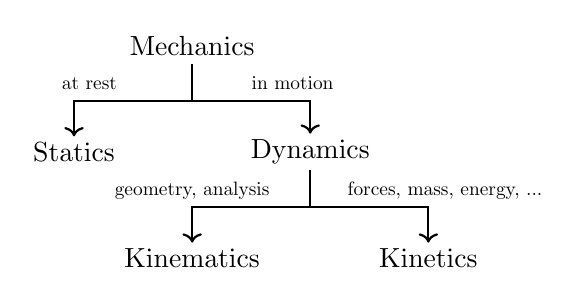
\begin{tikzpicture} %[xscale=1.3,yscale=1.3]
  \def\L{1.5}
  \def\H{2.7}
  \node[inner sep=3] %[draw=mydarkblue,thick,rounded corners=0.4,inner sep=2]
    (M) at (0,\H) {Mechanics};
  \node[inner sep=2]
    (S) at (-\L,0.5*\H) {Statics};
  \node[inner sep=2]
    (D) at (\L,0.5*\H) {Dynamics};
  \node[inner sep=2]
    (K) at (0.0*\L,0) {Kinematics};
  \node[inner sep=2]
    (k) at (2.0*\L,0) {Kinetics};
  \draw[->,thick] (M) --++ (0,-0.26*\H) -| (S)
    node[midway,left=6,above right=-1,scale=0.7] {\strut at rest}; %stationary};
  \draw[->,thick] (M) --++ (0,-0.26*\H) -| (D)
    node[midway,right=10,above left=-1,scale=0.7] {\strut in motion};
  \draw[->,thick] (D) --++ (0,-0.26*\H) -| (K)
    node[midway,left=0,above=-1,scale=0.7] {\strut geometry, analysis};
  \draw[->,thick] (D) --++ (0,-0.26*\H) -| (k)
    node[midway,right=6,above=-1,scale=0.7] {\strut forces, mass, energy, ...};
    \label{mechanics-flowchart}
\end{tikzpicture}
\endgroup

% Pendulum
\begingroup
% ref: https://tikz.net/dynamics_pendulum/
% Author: Izaak Neutelings (October 2020)
% Instructions: To compile, include data files from
%   https://github.com/IzaakWN/CodeSnippets/tree/master/LaTeX/TikZ/physics/dynamics_pendulum
% Other sources:
%   https://www.scielo.br/scielo.php?script=sci_arttext&pid=S1806-11172007000400024
%   https://www.researchgate.net/publication/262746594_Exact_solution_for_the_nonlinear_pendulum
%   https://tex.stackexchange.com/questions/545590/phase-portrait-of-van-der-pol-oscillator-with-pgfplots
%   http://matlab.cheme.cmu.edu/2011/08/09/phase-portraits-of-a-system-of-odes/
\tikzset{>=latex} % for LaTeX arrow head
\contourlength{1.2pt}

\colorlet{xcol}{blue!70!black}
\colorlet{vcol}{green!60!black}
\colorlet{myred}{red!70!black}
\colorlet{myblue}{blue!70!black}
\colorlet{mygreen}{green!70!black}
\colorlet{mydarkred}{myred!70!black}
\colorlet{mydarkblue}{myblue!60!black}
\colorlet{mydarkgreen}{mygreen!60!black}
\colorlet{acol}{red!50!blue!80!black!80}
\tikzstyle{CM}=[red!40!black,fill=red!80!black!80]
\tikzstyle{xline}=[xcol,thick,smooth]
\tikzstyle{mass}=[line width=0.6,red!30!black,fill=red!40!black!10,rounded corners=1,
                  top color=red!40!black!20,bottom color=red!40!black!10,shading angle=20]
\tikzstyle{faded mass}=[dashed,line width=0.1,red!30!black!40,fill=red!40!black!10,rounded corners=1,
                        top color=red!40!black!10,bottom color=red!40!black!10,shading angle=20]
\tikzstyle{rope}=[brown!70!black,very thick,line cap=round]
\def\rope#1{ \draw[black,line width=1.4] #1; \draw[rope,line width=1.1] #1; }
\tikzstyle{force}=[->,myred,very thick,line cap=round]
\tikzstyle{velocity}=[->,vcol,very thick,line cap=round]
\tikzstyle{Fproj}=[force,myred!40]
\tikzstyle{myarr}=[-{Latex[length=3,width=2]},thin]
\def\tick#1#2{\draw[thick] (#1)++(#2:0.12) --++ (#2-180:0.24)}
\def\N{80} % number of samples in plots

% PENDULUM
\def\L{2.8}  % string length
\def\diagramAngle{28} % angle string
\def\R{0.25} % ball radius
\def\F{1.0}  % force magnitude
\begin{tikzpicture}
  \message{^^JPendulum}
  \coordinate (M) at (\diagramAngle-90:\L);
  \coordinate (M') at (0,-\L);
  \coordinate (O) at (0,0);
  \coordinate (B) at (0,-\L-2.2*\R);
  \coordinate (FT) at ($(M)+(90+\diagramAngle:{\F*cos(\diagramAngle)+\R})$);
  \coordinate (FG) at ($(M)+(-90:{\F+\R})$);
  \coordinate (FGx) at ($(M)+(-90+\diagramAngle:{0.55*\F+\R})$);
  \coordinate (MA) at ($(M)+(180+\diagramAngle:{\F*sin(\diagramAngle)+\R})$);
  %\draw[faded mass] (M') circle(\R);
  \draw[<->] (M)++(\diagramAngle-32:0.2*\L) node[below right=-1,scale=0.9] {$x$}
    --++ (\diagramAngle:0.17*\L) --++ (90+\diagramAngle:0.17*\L) node[above right=-1,scale=0.9] {$y$};
  \draw[dashed] (O) -- (B);
  %\draw[dashed,myred!60!black] (MA) -- (FG);
  \draw[dashed,myred!60!black] (M) -- (FGx);
  \draw[dashed] (-90+\diagramAngle+10:\L) arc(-90+\diagramAngle+10:-110:\L) (B);
  \rope{(O) -- (M)} \path (O) -- (M) node[midway,above right=-1] {$L$};
  \fill[black] (O) circle(0.04);
  \draw[force] (M) -- (FT) node[midway,left=0] {$\bm{T}$};
  \draw[force] (M) -- (FG) node[right=0] {$m\bm{g}$};
  \draw[force,acol] (M) -- (MA) node[right=2,below=0] {$m\bm{a}$}; %{\contour{white}{$m\bm{a}$}};
  \draw[mass] (M) circle(\R) node {$m$};
  \draw pic[myarr,"$\theta$",xcol,draw=xcol,angle radius=22,angle eccentricity=1.30] {angle=B--O--M}; %_\text{max}
  \draw pic[myarr,"$\theta$",xcol,draw=xcol,angle radius=14,angle eccentricity=1.45] {angle=FG--M--FGx};
    \label{pendulum}
\end{tikzpicture}

% PENDULUM FORCES - ma
\begin{tikzpicture}
  \message{^^JPendulum forces}
  \def\F{1.4}  % force magnitude
  \coordinate (O) at (0,0);
  \coordinate (FT) at (90+\diagramAngle:{\F*cos(\diagramAngle)});
  \coordinate (FG) at (-90:\F);
  \coordinate (FGx) at (-90+\diagramAngle:{0.7*\F});
  \coordinate (MA) at (180+\diagramAngle:{\F*sin(\diagramAngle)});
  \draw[dashed,myred!60!black] (O) -- (FGx);
  \draw[dashed,myred!60!black] (MA) -- (FG);
  \draw[force] (O) -- (FT) node[midway,above right=-2] {$\bm{T}$};
  \draw[force] (O) -- (FG) node[right=0] {$m\bm{g}$};
  \draw[force,acol] (O) -- (MA) node[left=0] {$m\bm{a}$};
  \draw pic[myarr,"$\theta$",xcol,draw=xcol,angle radius=14,angle eccentricity=1.45] {angle=FG--O--FGx};
    \label{pendulum-acceleration}
\end{tikzpicture}

% PENDULUM FORCES
\begin{tikzpicture}
  \message{^^JPendulum forces}
  \def\F{1.4}  % force magnitude
  \coordinate (O) at (0,0);
  \coordinate (FT) at (90+\diagramAngle:{\F*cos(\diagramAngle)});
  \coordinate (FG) at (-90:\F);
  \coordinate (FGx) at (-90+\diagramAngle:{\F*cos(\diagramAngle)});
  \coordinate (FGy) at (180+\diagramAngle:{\F*sin(\diagramAngle)});
  \draw[dashed,myred!60!black] (FGy) -- (FG); %-- (FGx);
  \draw[force] (O) -- (FT) node[midway,above right=-2] {$\bm{T}$};
  \draw[Fproj] (O) -- (FGy) node[pos=0.4,above left=-3,scale=0.86] {$mg\sin\theta$};
  \draw[Fproj] (O) -- (FGx) node[pos=0.5,above right=-3,scale=0.86] {$mg\cos\theta$};
  \draw[force] (O) -- (FG) node[right=0] {$m\bm{g}$};
  \draw pic[myarr,"$\theta$",xcol,draw=xcol,angle radius=14,angle eccentricity=1.45] {angle=FG--O--FGx};
    \label{pendulum-forces}
\end{tikzpicture}

%% PENDULUM
%\begin{tikzpicture}
%  \coordinate (M) at (0,-\L);
%  \coordinate (O) at (0,0);
%  \rope{(O) -- (M)} \path (O) -- (M) node[midway,above right=-2] {$L$};
%  \fill[black] (O) circle(0.04);
%  \draw[velocity] (M)++(-\R,0) --++ (-2.7*\R,0) node[above=0] {$\bm{v}$};
%  \draw[mass] (M) circle(\R) node {$m$};
%\end{tikzpicture}

% PHYSICAL PENDULUM
\begin{tikzpicture}
  \message{^^JPhysical pendulum}
  \def\L{2.0}  % string length
  \def\diagramAngle{28} % angle string
  \def\R{0.25} % ball radius
  \def\F{1.3}  % force magnitude
  \coordinate (M) at (\diagramAngle-90:\L);
  \coordinate (R) at (\diagramAngle-90:1.1*\L);
  \coordinate (M') at (0,-\L);
  \coordinate (O) at (0,0);
  \coordinate (B) at (0,-\L-2.5*\R);
  \coordinate (FT) at (90:\F);
  \coordinate (FG) at ($(M)+(-90:\F)$);
  \coordinate (FGx) at ($(M)+(-90+\diagramAngle:{0.55*\F+\R})$);
  \coordinate (MA) at ($(M)+(180+\diagramAngle:{\F*sin(\diagramAngle)+\R})$);
  \draw[mass]
    (180:0.3*\L) to[out=90,in=180] (80:0.36*\L) to[out=0,in=90] (0:0.3*\L) to[out=-90,in=90]
    ($(R)+(0:0.7*\L)$) to[out=-90,in=0] ($(R)+(-90:0.4*\L)$) to[out=180,in=-90] ($(R)+(-180:0.6*\L)$) to[out=90,in=-90] cycle; %node {$m$};
  \draw[dashed] (O) -- (B);
  \draw[dashed] (O) -- (M);
  %\draw[dashed,myred!60!black] (MA) -- (FG);
  \draw[dashed] (-90+\diagramAngle+10:\L) arc(-90+\diagramAngle+10:-110:\L) (B);
  \fill[black] (O) circle(0.04);
  \draw[CM] (M) circle(0.09);
  \draw[force] (O) -- (FT) node[below right=0] {$\bm{F}_\mathrm{N}$};
  \draw[force] (M) -- (FG) node[right=0] {$M\bm{g}$};
%  \draw[force,acol] (M) -- (MA) node[right=2,below=0] {$m\bm{a}$}; %{\contour{white}{$m\bm{a}$}};
%  \draw pic[myarr,"$\theta$",xcol,draw=xcol,angle radius=22,angle eccentricity=1.30] {angle=B--O--M}; %_\text{max}
%  \draw pic[myarr,"$\theta$",xcol,draw=xcol,angle radius=14,angle eccentricity=1.45] {angle=FG--M--FGx};
    \label{physical-pendulum}
\end{tikzpicture}

%% EXACT SOLUTION
%% Other sources:
%%   https://www.scielo.br/scielo.php?script=sci_arttext&pid=S1806-11172007000400024
%%   https://www.researchgate.net/publication/262746594_Exact_solution_for_the_nonlinear_pendulum
%%   https://tex.stackexchange.com/questions/545590/phase-portrait-of-van-der-pol-oscillator-with-pgfplots
%%   http://matlab.cheme.cmu.edu/2011/08/09/phase-portraits-of-a-system-of-odes/
%% Instructions to compile this part of the code:
%%   These curves were generated numerically with these MATLAB scripts:
%%     https://github.com/IzaakWN/CodeSnippets/tree/master/LaTeX/TikZ/physics/dynamics_pendulum
%%   To compile this part of the code, the curves need to be loaded via external txt files.
%%   To download the txt files from GitHub via the command line, do e.g.
%%     wget https://github.com/IzaakWN/CodeSnippets/raw/master/LaTeX/TikZ/physics/dynamics_pendulum.zip
%%     unzip dynamics_pendulum.zip
%%   or
%%     svn checkout https://github.com/IzaakWN/CodeSnippets/trunk/LaTeX/TikZ/physics/dynamics_pendulum/data ./dynamics_pendulum/data
%\begin{tikzpicture}
%  \message{^^JPendulum exact solution}
%  \def\xmax{7.0}  % max x axis
%  \def\ymax{1.4}  % max y axis
%  \def\A{3.1*\ys} % amplitude, theta0 = 3.1 ~ 178°
%  \def\B{2.4*\ys} % amplitude, theta0 = 2.4 ~ 140°
%  \def\C{0.6*\ys} % amplitude, theta0 = 0.6 ~ 34.4°
%  \pgfmathsetmacro\Tb{\xmax/2.97}      % period, theta0 = 2.4 ~ 140°, T/T0 ~ 1.5602
%  \pgfmathsetmacro\Ta{\Tb*3.35/1.56}   % period, theta0 = 3.1 ~ 178°, T/T0 ~ 3.3485
%  \pgfmathsetmacro\Tc{\Tb*1.023/1.56}  % period, theta0 = 0.6 ~ 34.4°, T/T0 ~ 1.0230
%  \pgfmathsetmacro\xs{\Ta/(2*pi*3.35)} % xscale, note data uses T = 2*pi, omega0 = 1
%  \pgfmathsetmacro\ys{\ymax*0.28}      % yscale
%
%  % AXIS
%  \draw[->,thick] (0,-\ymax) -- (0,\ymax+0.2) node[above=-3] {$\theta$ [rad]};
%  \draw[->,thick] (-0.2,0) -- (\xmax+0.05,0) node[right=-1] {$t$ [s]};
%  \draw[mydarkblue!30,dashed]
%    (0, pi*\ys) --++ (0.90*\xmax,0)
%    node[right=1,scale=0.8] {$ \pi\,\unit{rad}= \ang{180}$}
%    (0,-pi*\ys) --++ (0.84*\xmax,0)
%    node[right=1,scale=0.8] {$-\pi\,\unit{rad}=-\ang{180}$};
%
%  % PLOT REAL PENDULUM
%  \begin{axis}[
%      axis lines=none,anchor=origin,x=1cm,y=1cm, % coincide with TikZ coordinates
%      xmin=0,xmax=0.94*\xmax/\xs,xscale=\xs,
%      y filter/.code={\pgfmathparse{\ys*\pgfmathresult}}
%    ]
%    \addplot[xline,mygreen] table {dynamics_pendulum/data/pendulum-0p6.txt};
%    \addplot[xline,myred] table {dynamics_pendulum/data/pendulum-2p4.txt};
%    \addplot[xline,xcol] table {dynamics_pendulum/data/pendulum-3p1.txt};
%  \end{axis}
%
%  % PLOT APPROXIMATION
%  \draw[xline,mydarkgreen,thin,dashed,samples=\N,smooth,variable=\x,domain=0:0.94*\xmax]
%    plot(\x,{\C*cos(360/\Tc*\x)});
%  \draw[xline,mydarkred,thin,dashed,samples=\N,smooth,variable=\x,domain=0:0.94*\xmax]
%    plot(\x,{\B*cos(360/\Tb*\x)});
%  \draw[xline,mydarkblue,thin,dashed,samples=\N,smooth,variable=\x,domain=0:0.94*\xmax]
%    plot(\x,{\A*cos(360/\Ta*\x)});
%
%  % TICKS
%  \tick{0, \A}{0} node[above=1,left=-1,scale=0.9,mydarkblue] {3.1}; %\ang{3.1}
%  \tick{0, \B}{0} node[below=0.5,left=-1,scale=0.9,mydarkred] {2.4};
%  \tick{0, \C}{0} node[below=0.5,left=-1,scale=0.9,mydarkgreen] {0.6};
%  \tick{0,-\A}{0} node[left=-1,scale=0.9,mydarkblue] {$-3.1$};
%  \tick{\Tb,0}{90} node[below,scale=0.9,mydarkred] {$T(2.4)$};
%  \tick{2*\Tb,0}{90} node[below,scale=0.9] {$2\color{mydarkred}{T(2.4)}$};
%
%\end{tikzpicture}
%
%
%% EXACT SOLUTION - angular velocity
%\begin{tikzpicture}
%  \message{^^JPendulum exact solution - dtheta/dt}
%  \def\xmax{7.0}   % max x axis
%  \def\ymax{1.4}   % max y axis
%  \def\wmax{2*\ys} % yscale
%  \pgfmathsetmacro\Ta{\xmax/2.97}      % period, theta0 = 2.4 ~ 140°, T/T0 ~ 1.5602
%  \pgfmathsetmacro\Tb{\Ta*3.35/1.56}   % period, theta0 = 3.1 ~ 178°, T/T0 ~ 3.3485
%  \pgfmathsetmacro\xs{\Tb/(2*pi*3.35)} % xscale, note data uses T = 2*pi, omega0 = 1
%  \pgfmathsetmacro\ys{\ymax*0.44}      % yscale
%  \pgfmathsetmacro\A{2*sin(deg(2.4/2))*\ys}  % amplitude, theta0 = 2.4 ~ 140°
%  \pgfmathsetmacro\B{2*sin(deg(3.1/2))*\ys}  % amplitude, theta0 = 3.1 ~ 178°
%
%  % AXIS
%  \draw[->,thick] (0,-\ymax) -- (0,\ymax+0.2) node[above=-3] {$\dot{\theta}$ [rad/s]};
%  \draw[->,thick] (-0.2,0) -- (\xmax+0.05,0) node[right=-1] {$t$ [s]};
%  \draw[mydarkblue!30,dashed]
%    (0, \wmax) --++ (0.9*\xmax,0) %node[right=1,scale=0.8] {$ \pi\,\unit{rad}= \ang{180}$}
%    (0,-\wmax) --++ (0.9*\xmax,0); %node[right=1,scale=0.8] {$-\pi\,\unit{rad}=-\ang{180}$};
%
%  % PLOT REAL PENDULUM
%  \begin{axis}[
%      axis lines=none,anchor=origin,x=1cm,y=1cm, % coincide with TikZ coordinates
%      xmin=0,xmax=0.94*\xmax/\xs,xscale=\xs,
%      y filter/.code={\pgfmathparse{\ys*\pgfmathresult}}
%    ]
%    \addplot[xline,myred]
%      table[y index=2] {dynamics_pendulum/data/pendulum-2p4.txt};
%    \addplot[xline,xcol]
%      table[y index=2] {dynamics_pendulum/data/pendulum-3p1.txt};
%  \end{axis}
%
%  % PLOT APPROXIMATION
%  \draw[xline,mydarkred,thin,dashed,samples=\N,smooth,variable=\x,domain=0:0.94*\xmax]
%    plot(\x,{-\A*sin(360/\Ta*\x)});
%  \draw[xline,mydarkblue,thin,dashed,samples=\N,smooth,variable=\x,domain=0:0.94*\xmax]
%    plot(\x,{-\B*sin(360/\Tb*\x)});
%
%  % TICKS
%  \tick{0, \wmax}{0} node[left=-2,scale=0.9] {$2\omega_0$};
%  \tick{0,-\wmax}{0} node[left=-2,scale=0.9] {$-2\omega_0$};
%  \tick{\Ta,0}{90} node[below,scale=0.9] {\contour{white}{$\color{mydarkred}{T(2.4)}$}};
%  \tick{2*\Ta,0}{90} node[below,scale=0.9] {\contour{white}{$2\color{mydarkred}{T(2.4)}$}};
%
%\end{tikzpicture}
%
%
%% EXACT SOLUTION
%\begin{tikzpicture}
%  \message{^^JPendulum exact solution (normalized)}
%  \def\xmax{7.0}  % max x axis
%  \def\ymax{1.4}  % max y axis
%  \def\A{3.1*\ys} % amplitude, theta0 = 3.1 ~ 178°
%  \def\B{2.4*\ys} % amplitude, theta0 = 2.4 ~ 140°
%  \def\C{1.6*\ys} % amplitude, theta0 = 1.6 ~ 91.7
%  \pgfmathsetmacro\T{0.95*\xmax/2} % period
%  \pgfmathsetmacro\ys{\ymax*0.28}  % yscale
%
%  % AXIS
%  \draw[->,thick] (0,-\ymax) -- (0,\ymax+0.2) node[above=-3] {$\theta$ [rad]};
%  \draw[->,thick] (-0.2,0) -- (\xmax+0.05,0) node[right=-1] {$t$ [s]};
%  \draw[mydarkblue!30,dashed]
%    (0, pi*\ys) --++ (0.98*\xmax,0) node[right=1,scale=0.8] {$ \pi\,\unit{rad}= \ang{180}$}
%    (0,-pi*\ys) --++ (0.90*\xmax,0) node[right=1,scale=0.8] {$-\pi\,\unit{rad}=-\ang{180}$};
%
%  % PLOT REAL PENDULUM
%  \begin{axis}[
%      axis lines=none,anchor=origin,x=1cm,y=1cm, % coincide with TikZ coordinates
%      xmin=0,xscale=\T, %0.94*7/3, %xmax=0.94*\xmax/\xs,
%      y filter/.code={\pgfmathparse{\ys*\pgfmathresult}}
%    ]
%    \addplot[xline,mygreen] table {dynamics_pendulum/data/pendulum-1p6_norm.txt};
%    \addplot[xline,myred] table {dynamics_pendulum/data/pendulum-2p4_norm.txt};
%    \addplot[xline,xcol] table {dynamics_pendulum/data/pendulum-3p1_norm.txt};
%  \end{axis}
%
%  % PLOT APPROXIMATION
%  \draw[xline,mydarkblue,thin,dashed,samples=\N,smooth,variable=\x,domain=0:0.94*\xmax]
%    plot(\x,{\A*cos(360/\T*\x)});
%  \draw[xline,mydarkred,thin,dashed,samples=\N,smooth,variable=\x,domain=0:0.94*\xmax]
%    plot(\x,{\B*cos(360/\T*\x)});
%  \draw[xline,mydarkgreen,thin,dashed,samples=\N,smooth,variable=\x,domain=0:0.94*\xmax]
%    plot(\x,{\C*cos(360/\T*\x)});
%
%  % TICKS
%  \tick{0, \A}{0} node[above=1,left=-1,scale=0.9] {\color{mydarkblue}{3.1}};
%  \tick{0, \B}{0} node[below=0.5,left=-1,scale=0.9] {\color{mydarkred}{2.4}};
%  \tick{0, \C}{0} node[below=0.5,left=-1,scale=0.9] {\color{mydarkgreen}{1.6}};
%  \tick{0,-\A}{0} node[left=-1,scale=0.9] {\color{mydarkblue}{$-3.1$}};
%  \tick{\T,0}{90} node[below,scale=0.9] {$T$};
%  \tick{2*\T,0}{90} node[below,scale=0.9] {$2T$};
%
%\end{tikzpicture}
%
%
%% EXACT SOLUTION - angular velocity
%\begin{tikzpicture}
%  \message{^^JPendulum exact solution - dtheta/dt (normalized)}
%  \def\xmax{7.0}   % max x axis
%  \def\ymax{1.4}   % max y axis
%  \def\wmax{2*\ys} % yscale
%  \pgfmathsetmacro\T{0.95*\xmax/2} % period
%  \pgfmathsetmacro\ys{\ymax*0.44}  % yscale
%  \pgfmathsetmacro\A{2*sin(deg(3.1/2))*\ys}  % amplitude, theta0 = 3.1 ~ 178°
%  \pgfmathsetmacro\B{2*sin(deg(2.4/2))*\ys}  % amplitude, theta0 = 2.4 ~ 140°
%  \pgfmathsetmacro\C{2*sin(deg(1.6/2))*\ys}  % amplitude, theta0 = 1.6 ~ 91.7°
%
%  % AXIS
%  \draw[->,thick] (0,-\ymax) -- (0,\ymax+0.2) node[above=-3] {$\dot{\theta}$ [rad/s]};
%  \draw[->,thick] (-0.2,0) -- (\xmax+0.05,0) node[right=-1] {$t$ [s]};
%  \draw[mydarkblue!30,dashed]
%    (0, \wmax) --++ (0.9*\xmax,0) %node[right=1,scale=0.8] {$ \pi\,\unit{rad}= \ang{180}$}
%    (0,-\wmax) --++ (0.9*\xmax,0); %node[right=1,scale=0.8] {$-\pi\,\unit{rad}=-\ang{180}$};
%
%  % PLOT REAL PENDULUM
%  \begin{axis}[
%      axis lines=none,anchor=origin,x=1cm,y=1cm, % coincide with TikZ coordinates
%      xmin=0,xscale=\T,
%      y filter/.code={\pgfmathparse{\ys*\pgfmathresult}}
%    ]
%    \addplot[xline,xcol]
%      table[y index=2] {dynamics_pendulum/data/pendulum-3p1_norm.txt};
%    \addplot[xline,myred]
%      table[y index=2] {dynamics_pendulum/data/pendulum-2p4_norm.txt};
%    \addplot[xline,mygreen]
%      table[y index=2] {dynamics_pendulum/data/pendulum-1p6_norm.txt};
%  \end{axis}
%
%  % PLOT APPROXIMATION
%  \draw[xline,mydarkblue,thin,dashed,samples=\N,smooth,variable=\x,domain=0:0.94*\xmax]
%    plot(\x,{-\A*sin(360/\T*\x)});
%  \draw[xline,mydarkred,thin,dashed,samples=\N,smooth,variable=\x,domain=0:0.94*\xmax]
%    plot(\x,{-\B*sin(360/\T*\x)});
%  \draw[xline,mydarkgreen,thin,dashed,samples=\N,smooth,variable=\x,domain=0:0.94*\xmax]
%    plot(\x,{-\C*sin(360/\T*\x)});
%
%  % LABELS
%  \node[above=0,scale=0.8,mydarkblue] at (0.78*\T,0.99*\A) {$\theta_0=3.1$};
%  \node[right,scale=0.8,mydarkred] at (0.81*\T,0.88*\B) {\contour{white}{$\theta_0=2.4$}};
%  \node[right,scale=0.8,mydarkgreen] at (0.96*\T,0.4*\C) {$\theta_0=1.6$};
%
%  % TICKS
%  \tick{0, \wmax}{0} node[left=-2,scale=0.9] {$2\omega_0$};
%  \tick{0,-\wmax}{0} node[left=-2,scale=0.9] {$-2\omega_0$};
%  \tick{\T,0}{90} node[left=2,below,scale=0.9] {$T$};
%  \tick{2*\T,0}{90} node[below,scale=0.9] {$2\color{mydarkred}{T}$};
%
%\end{tikzpicture}
%
%
%% EXACT SOLUTION - T/T0
%% https://en.wikipedia.org/wiki/Pendulum_(mathematics)
%\begin{tikzpicture}[xscale=1.1]
%  \message{^^JPendulum exact solution period (closed/bounded)}
%  \def\xmax{4.1}   % max x axis
%  \def\ymax{3.2}   % max y axis
%  \def\ys{0.82}    % yscale
%  \def\xs{1.02}    % xscale
%  \def\yz{\ys*0.4} % y zero
%  \def\xtick#1{\draw[thick] (#1)++(0,0.11) --++ (0,-0.22)}
%  \def\ytick#1{\draw[thick] (#1)++(0.1,0) --++ (-0.2,0)}
%
%  % AXIS
%  \draw[->,thick]
%    (0,\yz-0.1*\ymax) -- (0,\ymax+0.1) node[below=3,left=1] {$\dfrac{T}{T_0}$};
%  \draw[->,thick]
%    (-0.1*\ymax,\yz) -- (\xmax,\yz) node[right=3,below=0] {$\theta_0$ [rad]};
%  \draw[dashed] (\xs*pi,\yz) --++ (0,\ymax-\yz);
%
%  % REAL PENDULUM
%  \begin{axis}[
%      axis lines=none,anchor=origin,
%      x=1cm,y=1cm,ymin=0,ymax=\ymax,xscale=\xs,
%      y filter/.code={\pgfmathparse{\ys*\pgfmathresult}}
%    ]
%    \addplot[xline]
%      table[x index=0,y index=1] {dynamics_pendulum/data/pendulum_period.txt};
%  \end{axis}
%
%  % LINES
%  \draw[dashed,mydarkgreen]
%    (0,\ys) --++ (0.82*\xmax,0)
%    node[right=1,scale=0.8,align=left] {small-angle\\[-1mm]approximation};
%  \draw[dashed,mydarkred]
%    (0,\ys*1.18) -| (0.50*pi,\yz);
%
%  % TICKS
%  \xtick{0.25*\xs*pi,\yz} node[below=1,scale=0.9] {$\dfrac{\pi}{4}$};
%  \xtick{0.50*\xs*pi,\yz} node[below=1,scale=0.9] {$\dfrac{\pi}{2}$};
%  \xtick{0.75*\xs*pi,\yz} node[below=-0.9,scale=0.9] {$\dfrac{3\pi}{4}$};
%  \xtick{     \xs*pi,\yz} node[below=1,scale=0.9] {$\pi$};
%  \ytick{0,\ys} node[below=1.5,left=0,scale=0.9] {1};
%  \ytick{0,\ys*1.18} node[above=3,left=0,scale=0.8,mydarkred] {1.18};
%  \ytick{0,\ys*2} node[left=0,scale=0.9] {2};
%  \ytick{0,\ys*3} node[left=0,scale=0.9] {3};
%
%\end{tikzpicture}
%
%
%% EXACT SOLUTION - OPEN TRAJECTORY
%\begin{tikzpicture}
%  \message{^^JPendulum exact solution (open/unbounded, normalized)}
%  \def\xmax{7.0} % max x axis
%  \def\ymax{2.8} % max y axis
%  \pgfmathsetmacro\T{0.98*\xmax/2.5} % period
%  \pgfmathsetmacro\ys{\ymax*0.06}    % yscale
%
%  % AXIS
%  \draw[->,thick] (0,-0.2) -- (0,\ymax+0.2) node[above=-3] {$\theta$ [rad]};
%  \draw[->,thick] (-0.2,0) -- (\xmax+0.25,0) node[right=-1] {$t$ [s]};
%  \draw[mydarkblue!30,dashed,yscale=\ys]
%    (0,pi) --++ (\xmax,0)
%    (0,3*pi) --++ (\xmax,0)
%    (0,5*pi) --++ (\xmax,0);
%
%  % PLOT REAL PENDULUM
%  \begin{axis}[
%      axis lines=none,anchor=origin,x=1cm,y=1cm, % coincide with TikZ coordinates
%      xmin=0,xscale=\T, %0.94*7/3, %xmax=0.94*\xmax/\xs,
%      y filter/.code={\pgfmathparse{\ys*\pgfmathresult}}
%    ]s
%    \addplot[xline,xcol] table {dynamics_pendulum/data/pendulum_open-2p00000002_norm.txt};
%    \addplot[xline,myred] table {dynamics_pendulum/data/pendulum_open-2p01_norm.txt};
%    \addplot[xline,mygreen] table {dynamics_pendulum/data/pendulum_open-2p6_norm.txt};
%  \end{axis}
%
%  % LABELS
%  \node[above right=-1,scale=0.8,mydarkblue] at (0.97*\T,\ys*pi) {$\Omega_0/2\omega_0=1.00000001$};
%  %\node[right=2,scale=0.8,mydarkred] at (\T,1.96*\ys*pi) {\contour{white}{$\Omega_0/2\omega_0=1.005$}};
%  \node[below right=0,scale=0.8,mydarkred] at (1.27*\T,3*\ys*pi) {\contour{white}{$\Omega_0/2\omega_0=1.005$}};
%  %\node[below right=-1,scale=0.8,mydarkgreen] at (1.4*\T,3*\ys*pi) {$\Omega_0/2\omega_0=1.3$};
%  \node[below right=0,scale=0.8,mydarkgreen] at (2.01*\T,4.24*\ys*pi) {$\Omega_0/2\omega_0=1.3$};
%
%  % TICKS
%  \tick{0,pi*\ys}{0} node[left=-1,scale=0.9] {$\pi$};
%  \tick{0,2*pi*\ys}{0} node[left=-1,scale=0.9] {$2\pi$};
%  \tick{0,3*pi*\ys}{0} node[left=-1,scale=0.9] {$3\pi$};
%  \tick{0,4*pi*\ys}{0} node[left=-1,scale=0.9] {$4\pi$};
%  \tick{0,5*pi*\ys}{0} node[left=-1,scale=0.9] {$5\pi$};
%  \tick{\T,0}{90} node[below,scale=0.9] {$T$};
%  \tick{2*\T,0}{90} node[below,scale=0.9] {$2T$};
%
%\end{tikzpicture}
%
%
%% EXACT SOLUTION - OPEN TRAJECTORIES - T/T0
%% https://en.wikipedia.org/wiki/Pendulum_(mathematics)
%\begin{tikzpicture}
%  \message{^^JPendulum exact solution period (open/unbounded)}
%  \def\xmax{6.1} % max x axis
%  \def\ymax{2.9} % max y axis
%  \def\ys{2.2}   % yscale
%  \def\xs{0.79}   % xscale
%  \def\xtick#1{\draw[thick] (#1)++(0,0.11) --++ (0,-0.22)}
%  \def\ytick#1{\draw[thick] (#1)++(0.12,0) --++ (-0.24,0)}
%
%  % AXIS
%  \draw[->,thick] (0,-0.1*\ymax) -- (0,\ymax+0.2) node[below=3,left=1] {$\dfrac{T}{T_0}$};
%  \draw[->,thick] (-0.1*\xs*\ymax,0) -- (\xs*\xmax,0) node[right=3,below=0] {$\Omega_0/2\omega_0$};
%  %\draw[dashed] (pi,0) --++ (0,\ymax-0);
%
%  % UNIFORM MOTION
%  \draw[xline,mydarkgreen,thin,dashed,samples=\N,smooth,variable=\x,domain=\ys/(2.05*\ymax):5]
%    plot(\xs*\x,{\ys/(2*\x)});
%  \node[mydarkgreen,scale=0.75,above right=-4]
%    at (0.12,\ymax) {uniform circular motion, $\dfrac{T}{T_0}=\dfrac{\omega_0}{\Omega_0}$};
%
%  % REAL PENDULUM
%  \begin{axis}[
%      axis lines=none,anchor=origin,
%      x=1cm,y=1cm,ymin=0,ymax=\ymax,xmin=0,xmax=5,xscale=\xs,
%      y filter/.code={\pgfmathparse{\ys*\pgfmathresult}}
%    ]
%    \addplot[xline]
%      table[x index=1,y index=2] {dynamics_pendulum/data/pendulum_period_open.txt};
%  \end{axis}
%
%  % LINES
%  \draw[dashed,mydarkblue] (\xs,0) --++ (0,0.95*\ymax);
%
%  % TICKS
%  \xtick{\xs*1,0} node[below=1,scale=0.9] {$1$};
%  \xtick{\xs*2,0} node[below=1,scale=0.9] {$2$};
%  \xtick{\xs*3,0} node[below=1,scale=0.9] {$3$};
%  \xtick{\xs*4,0} node[below=1,scale=0.9] {$4$};
%  \xtick{\xs*5,0} node[below=1,scale=0.9] {$5$};
%  \ytick{0,\ys*0.5} node[below=1.5,left=0,scale=0.9] {$0.5$};
%  \ytick{0,\ys} node[below=1.5,left=0,scale=0.9] {$1$};
%
%\end{tikzpicture}

% PENDULUM EQUATIONS - CLOSED TRAJECTORIES
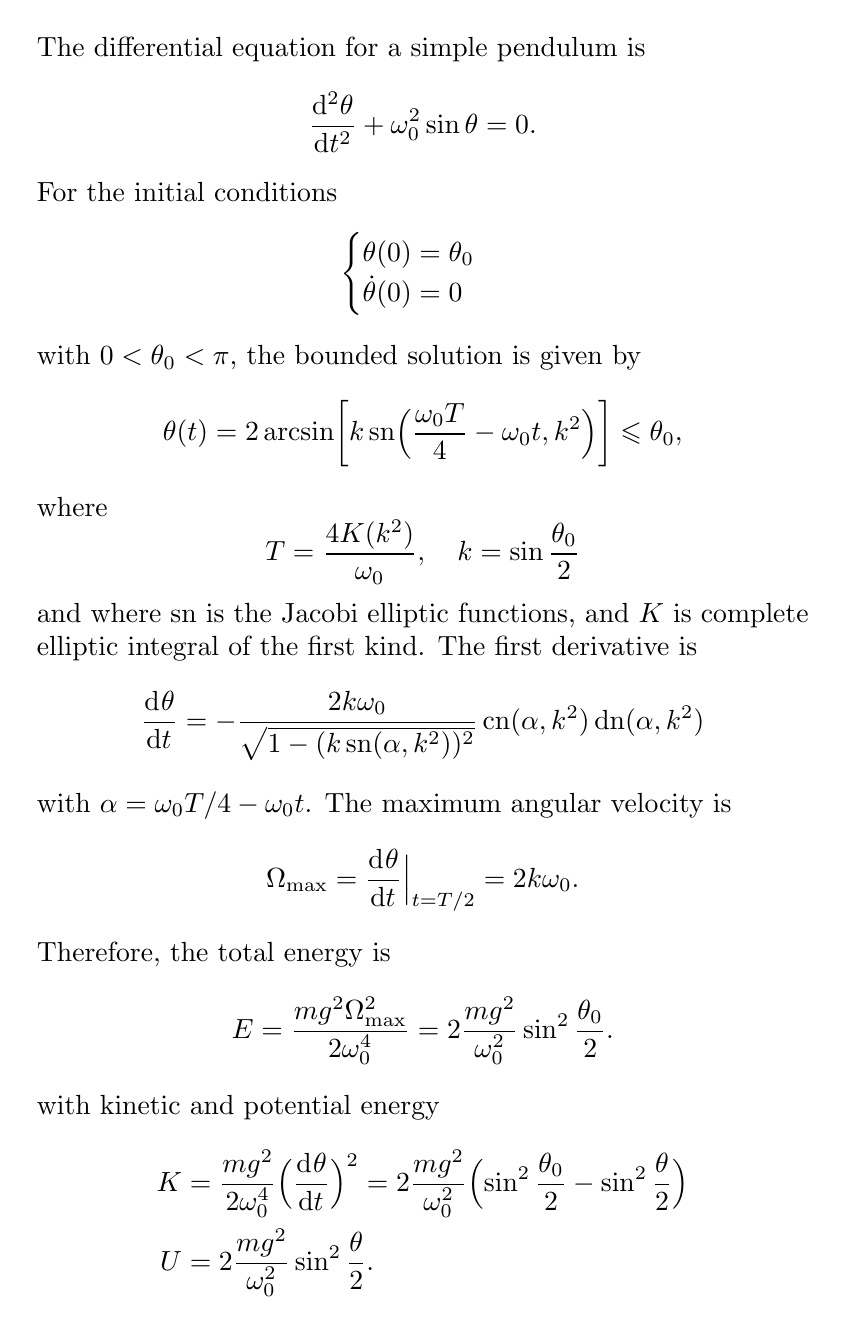
\begin{tikzpicture}[scale=1]
  \message{^^JPendulum equations (closed/bounded)}
  \def\myarg{(\alpha,k^2)}
  \node[align=left] at (0,0) {
    \begin{minipage}{9.8cm}
      The differential equation for a simple pendulum is
      \begin{equation*}
        \dv[2]{\theta}{t} + \omega_0^2\sin\theta = 0.
      \end{equation*}
      For the initial conditions
      \begin{equation*}
        \begin{cases}
          \theta(0) = \theta_0\\
          \dot\theta(0) = 0
        \end{cases}
      \end{equation*}
      with $0 < \theta_0 < \pi$,
      the bounded solution is given by
      \begin{equation*}
        \theta(t)
        = 2\arcsin\biggl[k\sn\Bigl(\frac{\omega_0T}{4} - \omega_0t,k^2\Bigr)\biggr]
        \leq \theta_0,
      \end{equation*}
      where
      \begin{equation*}
        %0<\theta_0<\pi,\quad
        T = \frac{4K(k^2)}{\omega_0},\quad
        k = \sin{\frac{\theta_0}{2}}
      \end{equation*}
      and where $\sn$ is the Jacobi elliptic functions,
      and $K$ is complete elliptic integral of the first kind.
      The first derivative is
      \begin{equation*}
        \dv{\theta}{t}
        = -\frac{2 k \omega_0}{\sqrt{1 - (k \sn\myarg)^2}} \cn\myarg\dn\myarg
      \end{equation*}
      with $\alpha = \omega_0T/4 - \omega_0t$.
      %\begin{equation*}
      %  \alpha = \frac{\omega_0T}{4}-\omega_0t.
      %\end{equation*}
      The maximum angular velocity is
      \begin{equation*}
        \Omega_{\max} = \dv{\theta}{t}\Bigr\rvert_{t=T/2} = 2k\omega_0.
      \end{equation*}
      Therefore, the total energy is
      \begin{equation*}
        E = \frac{mg^2\Omega_{\max}^2}{2\omega_0^4}
          = 2\frac{mg^2}{\omega_0^2}\sin^2\frac{\theta_0}{2}.
      \end{equation*}
      with kinetic and potential energy
      \begin{align*}
        K &= \frac{mg^2}{2\omega_0^4}\Bigl(\dv{\theta}{t}\Bigr)^2
           = 2\frac{mg^2}{\omega_0^2}\Bigl(\sin^2\frac{\theta_0}{2} - \sin^2\frac{\theta}{2}\Bigr) \\
        U &= 2\frac{mg^2}{\omega_0^2}\sin^2\frac{\theta}{2}.
      \end{align*}
     \end{minipage}
  };
    \label{pendulum-libration-equations}
\end{tikzpicture}

% PENDULUM EQUATIONS - OPEN TRAJECTORIES
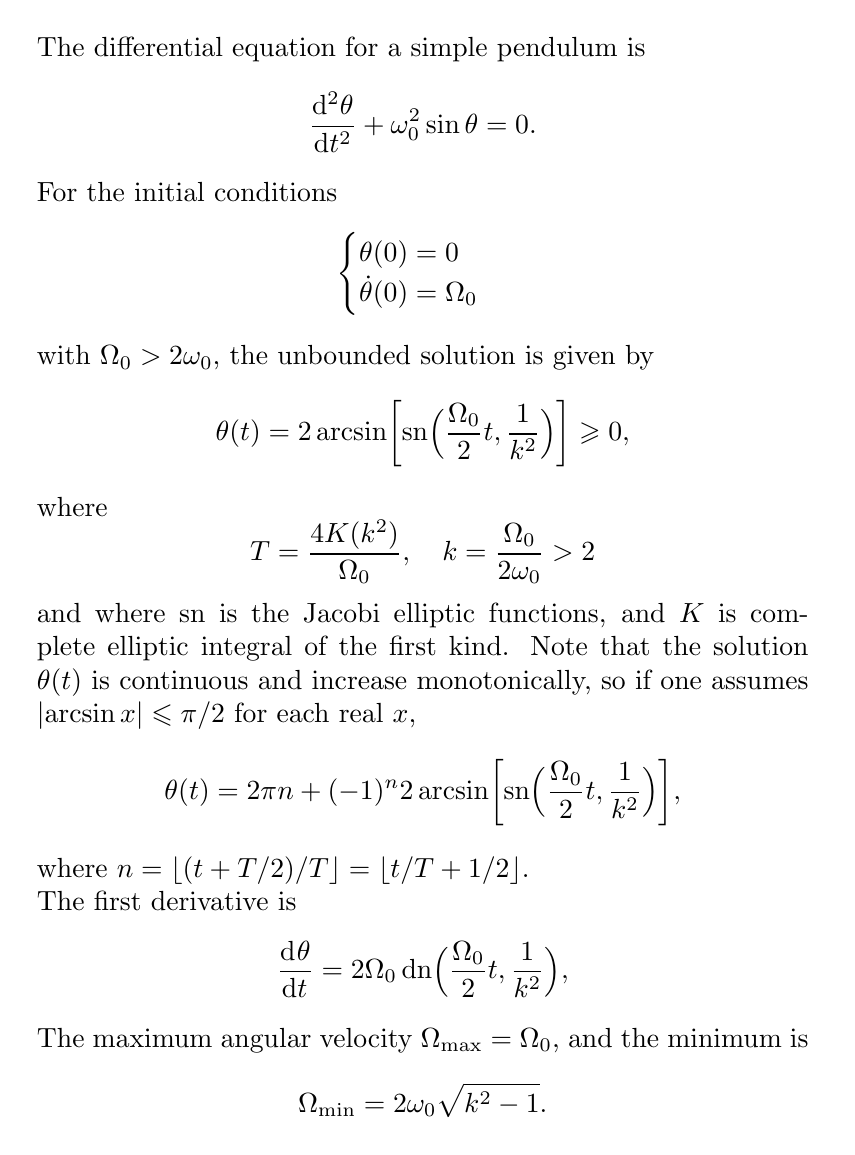
\begin{tikzpicture}[scale=1]
  \message{^^JPendulum equations (open/unbounded)}
  \def\myarg{\Bigl(\frac{\Omega_0}{2}t,\frac{1}{k^2}\Bigr)}
  \node[align=left] at (0,0) {
    \begin{minipage}{9.8cm}
      The differential equation for a simple pendulum is
      \begin{equation*}
        \dv[2]{\theta}{t} + \omega_0^2\sin\theta = 0.
      \end{equation*}
      For the initial conditions
      \begin{equation*}
        \begin{cases}
          \theta(0) = 0 \\
          \dot\theta(0) = \Omega_0 %> 2\omega_0
        \end{cases}
      \end{equation*}
      with $\Omega_0 > 2\omega_0$,
      the unbounded solution is given by
      \begin{equation*}
        \theta(t)
        = 2\arcsin\biggl[\sn\myarg\biggr]
        \geq 0,
      \end{equation*}
      where
      \begin{equation*}
        %\Omega_0 > 2\omega_0,\quad
        T = \frac{4K(k^2)}{\Omega_0},\quad
        k = \frac{\Omega_0}{2\omega_0} > 2
      \end{equation*}
      and where sn is the Jacobi elliptic functions,
      and $K$ is complete elliptic integral of the first kind.
      Note that the solution $\theta(t)$ is continuous and increase monotonically,
      so if one assumes $\lvert\arcsin x\rvert \leq \pi/2$ for each real $x$,
      \begin{equation*}
        \theta(t)
        = 2\pi n + (-1)^n 2\arcsin\biggl[\sn\myarg\biggr],
      \end{equation*}
      where $n = \lfloor(t + T/2)/T\rfloor = \lfloor t/T + 1/2\rfloor$.\\
      The first derivative is
      \begin{equation*}
        \dv{\theta}{t} = 2\Omega_0\dn\myarg,
      \end{equation*}
      The maximum angular velocity $\Omega_{\max} = \Omega_0$,
      and the minimum is
      \begin{equation*}
        \Omega_{\min} = 2\omega_0\sqrt{k^2 - 1}.
      \end{equation*}
    \end{minipage}
  };
    \label{pendulum-rotation-equations}
\end{tikzpicture}
\endgroup

% Complex oscillations
\begingroup
% ref: https://tikz.net/complex/
% Author: Izaak Neutelings (January 2021)


%\usetikzlibrary{intersections}
%\usetikzlibrary{decorations.markings}
\contourlength{1.0pt}

\tikzset{>=latex} % for LaTeX arrow head
\colorlet{myblue}{blue!65!black}
\colorlet{mydarkblue}{blue!50!black}
\colorlet{myred}{red!65!black}
\colorlet{mydarkred}{red!40!black}
\colorlet{veccol}{green!70!black}
\colorlet{vcol}{green!70!black}
\colorlet{xcol}{blue!85!black}
%\colorlet{projcol}{xcol!60}
%\colorlet{unitcol}{xcol!60!black!85}
%\colorlet{myred}{red!90!black}
%\colorlet{mypurple}{blue!50!red!80!black!80}
\tikzstyle{vector}=[->,very thick,xcol,line cap=round]
\tikzstyle{xline}=[myblue,very thick]
\tikzstyle{yzp}=[canvas is zy plane at x=0]
\tikzstyle{xzp}=[canvas is xz plane at y=0]
\tikzstyle{xyp}=[canvas is xy plane at z=0]
\def\tick#1#2{\draw[thick] (#1) ++ (#2:0.12) --++ (#2-180:0.24)}
\def\N{100}

% COMPLEX
\begin{tikzpicture}
  \def\xmax{2.0}
  \def\ymax{1.6}
  \def\R{1.9}
  \def\diagramAngle{35}
  \coordinate (O) at (0,0);
  \coordinate (R) at (\diagramAngle:\R);
  \coordinate (-R) at (-\diagramAngle:\R);
  \coordinate (X) at ({\R*cos(\diagramAngle)},0);
  \coordinate (Y) at (0,{\R*sin(\diagramAngle)});
  \coordinate (-Y) at (0,{-\R*sin(\diagramAngle)});
  \node[fill=mydarkblue,circle,inner sep=0.8] (R') at (R) {};
  \node[fill=mydarkred,circle,inner sep=0.8] (-R') at (-R) {};
  \node[mydarkblue,above right=-2] at (R') {$z = x + \i y = r\e^{\i\theta}$};
  \node[mydarkred,below right=-1] at (-R') {$\overline{z} = x - \i y = r\e^{-\i\theta}$};
  \draw[dashed,mydarkblue]
    (Y) -- (R') --++ (0,{0.1-\R*sin(\diagramAngle)});
  \draw[dashed,mydarkred]
    (-Y) -- (-R') --++ (0,{\R*sin(\diagramAngle)-0.45});
  \draw[->,line width=0.9] (-0.65*\xmax,0) -- (\xmax+0.05,0) node[right] {Re};
  \draw[->,line width=0.9] (0,-\ymax) -- (0,\ymax+0.05) node[left] {Im};
  \draw[vector] (O) -- (R') node[pos=0.55,above left=-2] {$r$};
  \draw[vector,myred] (O) -- (-R') node[pos=0.55,below left=-2] {$r$};
  \draw pic[->,"$\theta$",mydarkblue,draw=mydarkblue,angle radius=23,angle eccentricity=1.24]
    {angle = X--O--R};
  \draw pic[<-,"$-\theta$"{right=-1},mydarkred,draw=mydarkred,angle radius=20,angle eccentricity=1]
    {angle = -R--O--X};
  %\tick{X}{90} node[scale=0.9,left=6,below right=-2] {$x = r\cos\theta$};
  \tick{X}{90} node[scale=1,below=-1] {$x$};
  \tick{Y}{ 0} node[mydarkblue,scale=1,left] {$y$}; %r\sin\theta =
  \tick{-Y}{ 0} node[mydarkred,scale=1,left] {$-y$};
    \label{complex-plane}
\end{tikzpicture}

% COMPLEX numbers
\begin{tikzpicture}
  \def\xmax{1.7}
  \def\ymax{1.6}
  \def\re{0.7*\xmax}
  \def\im{0.7*\ymax}
  \coordinate (O) at (0,0);
  \draw[dashed,mydarkblue]
    (-\re,\im) -| (\re,-\im) -| cycle;
  \draw[->,line width=0.9] (-\xmax,0) -- (\xmax+0.1,0) node[right] {Re};
  \draw[->,line width=0.9] (0,-\ymax) -- (0,\ymax+0.1) node[left] {Im};
  \tick{\re,0}{90} node[mydarkblue,scale=1,below=-1] {\contour{white}{$1$}};
  \tick{-\re,0}{90} node[mydarkblue,scale=1,below=-1] {\contour{white}{$-1$}};
  \tick{0,\im}{ 0} node[mydarkblue,scale=1,left] {\contour{white}{$\i$}}; %r\sin\theta =
  \tick{0,-\im}{ 0} node[mydarkblue,scale=1,left] {\contour{white}{$-\i$}};
  \fill[mydarkblue]
    (   0, \im) circle(0.05)
    (   0,-\im) circle(0.05)
    ( \re,   0) circle(0.05)
    (-\re,  0) circle(0.05)
    ( \re, \im) circle(0.05)
      node[mydarkblue,scale=1,above right=-2] {\strut$1 + \i$}
    ( \re,-\im) circle(0.05)
      node[mydarkblue,scale=1,below right=-1] {\strut$1 - \i$}
    (-\re, \im) circle(0.05)
      node[mydarkblue,scale=1,above left=-2] {\strut$-1 + \i$}
    (-\re,-\im) circle(0.05)
      node[mydarkblue,scale=1,below left=-1] {\strut$-1 - \i$};
    \label{complex-numbers}
\end{tikzpicture}

% COMPLEX OSCILLATOR
\begin{tikzpicture}
  \def\xmax{2.2}
  \def\ymax{2.2}
  \def\R{1.8}
  \def\diagramAngle{35}
  \coordinate (O) at (0,0);
  \coordinate (R) at (\diagramAngle:\R);
  \coordinate (X) at ({\R*cos(\diagramAngle)},0);
  \coordinate (Y) at (0,{\R*sin(\diagramAngle)});
  \draw[xline] (O) circle (\R); %0.995*\R
  \node[fill=myred,circle,inner sep=1] (R') at (R) {};
  \node[mydarkblue,above right=0] at (R') {$z(t) = A\e^{\i\omega t}$};
  \draw[dashed,mydarkblue]
    (Y) -- (R') --++ (0,{0.1-\R*sin(\diagramAngle)});
  \draw[->,line width=0.9] (-\xmax,0) -- (\xmax+0.05,0) node[right] {Re};
  \draw[->,line width=0.9] (0,-\ymax) -- (0,\ymax+0.05) node[left] {Im};
  \draw[vector] (O) -- (R') node[pos=0.55,above left=-2] {$A$};
  \draw pic[->,"$\omega t$",mydarkblue,draw=mydarkblue,angle radius=22,angle eccentricity=1.4]
    {angle = X--O--R};
  \tick{0,\R+0.015}{0}; %node[scale=0.9,left=2] {\contour{white}{$R$}};
  \tick{\R+0.015,0}{90}; %node[scale=0.9,right=1,below=0] {\contour{white}{$R$}};
  \tick{0,-\R-0.015}{0};
  \tick{-\R-0.015,0}{90};
  \tick{X}{90} node[scale=0.9,left=14,below=-1] {$A\cos(\omega t)$}; %{\contour{white}{$A\cos(\omega t)$}};
  \tick{Y}{ 0} node[scale=0.9,below=1,left=-2] {$A\sin(\omega t)$}; % {\contour{white}{$A\sin(\omega t)$}};
    \label{complex-oscillator}
\end{tikzpicture}

% COMPLEX OSCILLATOR 3D
\def\xang{-13}
\def\zang{45}
\begin{tikzpicture}[x=(\xang:0.9), y=(90:0.9), z=(\zang:1.1)]
  \message{^^JSynthesis 3D}
  \def\xmax{8.8}         % max x axis
  \def\ymin{-1.5}        % min y axis
  \def\ymax{1.6}         % max y axis
  \def\zmax{1.6}         % max z axis
  \def\xf{1.17*\xmax}    % x position frequency axis
  \def\A{(0.70*\ymax)}   % amplitude
  \def\T{(0.335*\xmax)}  % period
  \def\w{\zmax/11.2}     % spacing components
  \def\diagramAngle{47}           % angle
  \def\s{\diagramAngle/360*\T}    % time component
  \def\x{\A*cos(\diagramAngle)}   % real component
  \def\y{\A*sin(\diagramAngle)}   % imaginary component

  % COMPLEX PLANE
  \begin{scope}[shift={(-1.6*\zmax,0,0)}]
    \draw[black,fill=white,opacity=0.3,yzp]
      (-1.25*\zmax,-1.25*\ymax) rectangle (1.4*\zmax,1.25*\ymax);
    \draw[->,thick] (0,\ymin,0) -- (0,\ymax+0.02,0)
      node[pos=1,left=0,yzp] {Im};
    \draw[->,thick] (0,0,-\zmax) -- (0,0,\zmax+0.02)
      node[right=1,below=0,yzp] {Re} coordinate (X);
    %\node[scale=1,yzp] at (0,-\ymax,0) {Complex plane};
    \draw[xline,yzp] (0,0) circle(0.991*\A) coordinate (O);
    \fill[myred,yzp] (\diagramAngle:{\A}) circle(0.07) coordinate(P);
    \node[mydarkblue,above=3,right=-5,yzp,scale=0.8] at (P) {$z(t) = A\e^{\i\omega t}$};
    \draw[vector,thick,yzp] (0,0) -- (\diagramAngle:{\A-0.03}) coordinate (R);
    \draw pic[-{>[flex'=1]},draw=mydarkblue,angle radius=14,angle eccentricity=1,
              "$\omega t$"{above=0,right=-0.5,yslant=0.69,scale=0.8},mydarkblue,yzp]
      {angle = X--O--R};
    \tick{0,0,{\A}}{90};
    \tick{0,0,{-\A}}{90};
    \tick{0,{\A},0}{\zang};
    \tick{0,{-\A},0}{\zang};
  \end{scope}

  % IMAGINARY
  \begin{scope}[shift={(0,0,1.9*\zmax)}]
    \draw[black,fill=white,opacity=0.3,xyp]
      (-0.5*\ymax,-1.2*\ymax) rectangle (1.10*\xmax,1.25*\ymax);
    \draw[->,thick] (-0.3*\ymax,0,0) -- (\xmax,0,0)
      node[below right=-2,xyp] {$t$};
    \draw[->,thick] (0,\ymin,0) -- (0,\ymax,0)
      node[left,xyp] {Im};
    \draw[xline,samples=\N,smooth,variable=\t,domain=-0.05*\T:0.95*\xmax]
      plot(\t,{\A*sin(360/\T*\t)},0);
    %\node[below=0,xyp] at (0.4*\xmax,-\ymax,0) {Imaginary component};
    \fill[myred,xyp] ({\s},{\y}) circle(0.07) coordinate(I);
    \draw[vector,thick,xyp] ({\s},0) --++ (0,{\y-0.03});
    \tick{0,{\A},0}{180};
    \tick{0,{-\A},0}{180};
    \tick{{\s},0,0}{90} node[right=0,below=-1,xyp] {$t$};
    \tick{{\T},0,0}{90} node[right=0,below,xyp] {\contour{white}{$T$}};
    \tick{{2*\T},0,0}{90} node[right=0,below,xyp] {\contour{white}{$2T$}};
    \node[mydarkblue,below=0,xyp] at (0.4*\xmax,1.15*\ymax,0) {$y(t) = A\sin(\omega t)$};
  \end{scope}

  % REAL
  \begin{scope}[shift={(0,-1.8*\zmax,0)}]
    \draw[black,fill=white,opacity=0.3,xzp]
      (-0.5*\ymax,-1.4*\ymax) rectangle (1.10*\xmax,1.25*\ymax);
    \draw[->,thick] (-0.3*\ymax,0,0) -- (\xmax,0,0)
      node[below right=-1,xzp] {$t$};
    \draw[->,thick] (0,0,-\zmax) -- (0,0,\zmax)
      node[left=-1,xzp] {Re};
    \draw[xline,samples=\N,smooth,variable=\t,domain=-0.05*\T:0.95*\xmax]
      plot(\t,0,{\A*cos(360/\T*\t)});
    %\node[below=0,xzp] at (0.4*\xmax,-\ymax,0) {Real component};
    \fill[myred,xzp] ({\s},{\x}) circle(0.07) coordinate(R);
    \draw[vector,thick,xzp] ({\s},0) --++ (0,{\x-0.03});
    \tick{0,0,{\A}}{180};
    \tick{0,0,{-\A}}{180};
    \tick{{\s},0,0}{\zang} node[below=-1,xzp] {$t$};
    \tick{{\T},0,0}{\zang} node[below,xzp] {$T$};
    \tick{{2*\T},0,0}{\zang} node[below,xzp] {$2T$};
    \node[mydarkblue,above=0,xzp] at (0.3*\xmax,-\ymax,0) {$x(t) = A\cos(\omega t)$};
  \end{scope}

  % COMPONENTS
  \draw[myred!80!black,dashed]
    (P) -- ({\s},{\y},{\x})
    (I) -- ({\s},{\y},{\x+0.05})
    ({\s},{\y-0.06},{\x}) -- (R);
  \draw[->,black,thick] (-0.1*\ymax,0,0) -- (\xmax,0,0) node[below right=-2] {$t$};
  \draw[->,black,thick] (0,\ymin,0) -- (0,\ymax+0.02,0) node[above] {Im};
  \draw[->,black,thick] (0,0,-\zmax) -- (0,0,\zmax+0.02) node[right=1,below=3] {Re};
  \foreach \i [evaluate={\tmin=max(-0.05*\T,(\i-0.05)*\T); \tmax=min(0.95*\xmax,(\i+1)*\T);}] in {0,...,2}{
    %\draw[white,line width=1.2] (\tmin,0,0) -- (\tmax,0,0);
    \draw[thick] (\tmin,0,0) -- (\tmax,0,0);
    \draw[xline,samples=0.4*\N,smooth,variable=\t]
      plot[domain=\tmin:\tmax](\t,{\A*sin(360/\T*\t)},{\A*cos(360/\T*\t)});
  }
  \draw[thick] (0,0,{0.9*\A}) -- (0,0,{\A});
  \fill[myred] ({\s},{\y},{\x}) circle(0.07) coordinate(Z);
  \draw[vector,thick] ({\s},0,0) --++ (0,{\y-0.03},{\x-0.03});
  \draw[xline,samples=0.3*\N,smooth,variable=\t,domain=\s+0.03:\s+0.4*\T,line cap=round]
    plot(\t,{\A*sin(360/\T*\t)},{\A*cos(360/\T*\t)});
  \tick{{\T},0,0}{90};
  \tick{{2*\T},0,0}{90};
  \tick{0,0,{\A}}{90};
  \tick{0,0,{-\A}}{90};
  \tick{0,{\A},0}{\zang};
  \tick{0,{-\A},0}{\zang};
  \draw[myred!80!black,dashed]
    ({\s},{\y-0.06},{\x}) --++ (0,-0.2*\ymax,0);

    \label{complex-oscillator-3d}
\end{tikzpicture}

% VECTOR ROTATION
\def\xmax{2.7}
\def\ymax{2.7}
\def\R{2.3}
\def\diagramAngle{28}
\def\dang{35}
\begin{tikzpicture}
  \coordinate (O) at (0,0);
  \coordinate (R) at (\diagramAngle:\R);
  \coordinate (Q) at (\diagramAngle+\dang:\R);
  \coordinate (X) at ({\R*cos(\diagramAngle)},0);
  \coordinate (Y) at (0,{\R*sin(\diagramAngle)});
  \coordinate (X') at ({\R*cos(\diagramAngle+\dang)},0);
  \coordinate (Y') at (0,{\R*sin(\diagramAngle+\dang)});
  %\draw[myblue] (O) circle (0.995*\R);
  \draw[myblue] (-10:\R) arc (-10:100:\R);
  \node[fill=myred,circle,inner sep=0.8] at (R) {};
  \node[fill=myred,circle,inner sep=0.8] at (Q) {};
  \node[mydarkblue,above right=-2] at (R) {$\bm{r} = (x,y)$};
  \node[mydarkblue,above right=-2] at (Q) {$\bm{r}' = (x',y')$};
  \draw[dashed,mydarkblue]
    (Y) -- (R) --++ (0,{0.1-\R*sin(\diagramAngle)});
  \draw[dashed,mydarkblue]
    (Y') -- (Q) --++ (0,{0.1-\R*sin(\diagramAngle+\dang)});
  \draw[->,line width=0.9] (-0.1*\xmax,0) -- (\xmax+0.05,0) node[right] {$x$};
  \draw[->,line width=0.9] (0,-0.1*\ymax) -- (0,\ymax+0.05) node[left] {$y$};
  \draw[vector] (O) -- (R);
  \draw[vector] (O) -- (Q);
  \draw pic[->,"$\phi$",mydarkblue,draw=mydarkblue,angle radius=20,angle eccentricity=1.35]
    {angle = R--O--Q};
  \tick{0,\R+0.015}{0};
  \tick{\R+0.015,0}{90};
  \tick{X}{90} node[scale=0.9,left=0,below=-1] {$x$};
  \tick{Y}{ 0} node[scale=0.9,below=1,left=-2] {$y$};
  \tick{X'}{90} node[scale=0.9,left=0,below=-4] {$x'$};
  \tick{Y'}{ 0} node[scale=0.9,below=1,left=-2] {$y'$};
    \label{vector-rotation}
\end{tikzpicture}

% COMPLEX ROTATION
\begin{tikzpicture}
  \coordinate (O) at (0,0);
  \coordinate (R) at (\diagramAngle:\R);
  \coordinate (Q) at (\diagramAngle+\dang:\R);
  \coordinate (X) at ({\R*cos(\diagramAngle)},0);
  \coordinate (Y) at (0,{\R*sin(\diagramAngle)});
  %\draw[myblue] (O) circle (0.995*\R);
  \draw[myblue] (-10:\R) arc (-10:100:\R);
  \node[fill=myred,circle,inner sep=0.8] at (R) {};
  \node[fill=myred,circle,inner sep=0.8] at (Q) {};
  \node[mydarkblue,above right=0] at (R) {$z = r\e^{\i\theta}$};
  \node[mydarkblue,left=2,above right=0] at (Q) {$z\e^{\i\phi} = r\e^{\i(\theta+\phi)}$};
  \draw[dashed,mydarkblue]
    (Y) -- (R) --++ (0,{0.1-\R*sin(\diagramAngle)});
  \draw[->,line width=0.9] (-0.1*\xmax,0) -- (\xmax+0.05,0) node[right] {Re};
  \draw[->,line width=0.9] (0,-0.1*\ymax) -- (0,\ymax+0.05) node[left] {Im};
  \draw[vector] (O) -- (R) node[pos=0.65,above left=-3] {$r$};
  \draw[vector] (O) -- (Q) node[pos=0.65,above left=-3] {$r$};
  \draw pic[->,"$\theta$",mydarkblue,draw=mydarkblue,angle radius=24,angle eccentricity=1.25]
    {angle = X--O--R};
  \draw pic[->,"$\phi$",mydarkblue,draw=mydarkblue,angle radius=20,angle eccentricity=1.35]
    {angle = R--O--Q};
  \tick{0,\R+0.015}{0};
  \tick{\R+0.015,0}{90};
  \tick{X}{90} node[scale=0.9,left=14,below=-1] {$r\cos\theta$};
  \tick{Y}{ 0} node[scale=0.9,below=1,left=-2] {$r\sin\theta$};
    \label{complex-rotation}
\end{tikzpicture}
\endgroup

% Rotating frames
\begingroup
% ref: https://tikz.net/reference_frame_rotational/
% author: Izaak Neutelings (September 2020)

\tikzset{>=latex} % for LaTeX arrow head
\contourlength{1.3pt}

\colorlet{xcol}{blue!70!black}
\colorlet{xcol'}{xcol!50!red}
\colorlet{vcol}{green!45!black}
\colorlet{acol}{red!50!blue!80!black!80}
\tikzstyle{rvec}=[->,very thick,xcol,line cap=round]
\tikzstyle{vvec}=[->,very thick,vcol,line cap=round]
\tikzstyle{avec}=[->,very thick,acol,line cap=round]
\colorlet{myred}{red!65!black}
\tikzstyle{force}=[->,myred,very thick,line cap=round]
\tikzstyle{mass}=[line width=0.5,draw=red!50!black,fill=red!50!black!10,rounded corners=1,
                  top color=red!50!black!30,bottom color=red!50!black!10,shading angle=20]
\tikzstyle{disk}=[line width=0.5,orange!30!black,fill=orange!40!black!10,
                  top color=orange!40!black!20,bottom color=orange!40!black!10,shading angle=20]
\tikzstyle{pole}=[line width=0.5,blue!20!black,fill=orange!20!black!10,
                  top color=blue!20!black!20,bottom color=blue!20!black!10,shading angle=20]
\tikzstyle{rope}=[brown!70!black,line width=1,line cap=round] %very thick
\tikzstyle{myarr}=[-{Latex[length=3,width=2,flex'=1]},thin]
\tikzstyle{mydashed}=[dash pattern=on 2pt off 1pt]
\def\rope#1{ \draw[rope,black,line width=1.4] #1; \draw[rope,line width=1.1] #1; }
\def\tick#1#2{\draw[thick] (#1) ++ (#2:0.1) --++ (#2-180:0.2)}
\newcommand\rightAngle[4]{
  \pgfmathanglebetweenpoints{\pgfpointanchor{#2}{center}}{\pgfpointanchor{#3}{center}}
  \coordinate (tmpRA) at ($(#2)+(\pgfmathresult+45:#4)$);
  %\draw[white,line width=0.6] ($(#2)!(tmpRA)!(#1)$) -- (tmpRA) -- ($(#2)!(tmpRA)!(#3)$);
  \draw[black] ($(#2)!(tmpRA)!(#1)$) -- (tmpRA) -- ($(#2)!(tmpRA)!(#3)$);
}

% ROTATION
\def\L{3.1}     % axis lengths
\def\R{1.0*\L}  % position vector radial distance
\def\Rang{52}   % position vector angle
\def\diagramAngle{25}    % angle of the CM velocity
\begin{tikzpicture}
  \coordinate (O) at (0,0);
  \coordinate (X) at (1.05*\L,0);
  \coordinate (Y) at (0,1.05*\L);
  \coordinate (X') at (\diagramAngle:\L);
  \coordinate (Y') at (90+\diagramAngle:\L);
  \coordinate (R) at (\Rang:\R);
  \node[fill=blue!40!black,circle,inner sep=0.9] (R') at (R) {};
  \node[above right=-1] at (R') {P};
  \coordinate (Rx) at (0:{\R*cos(\Rang)});
  \coordinate (Ry) at (90:{\R*sin(\Rang)}); %($(Y)!(O)!(R)$);
  \coordinate (Rx') at (\diagramAngle:{\R*cos(\Rang-\diagramAngle)});
  \coordinate (Ry') at (90+\diagramAngle:{\R*sin(\Rang-\diagramAngle)});

  % AXES
  \draw[<->,very thick,xcol!70!black]
    (X) node[right=-1,xcol] {$x$} -- (O) node[below left=-3] {O} --
    (Y) node[left=-1,xcol] {$y$};
  \draw[<->,very thick,xcol'!70!black]
    (X') node[above=2,right=-2,xcol'] {$x'$} -- (O) --
    (Y') node[left=-2,xcol'] {$y'$};

  % POSITION VECTOR
  \draw[rvec,vvec,line cap=round] (O) -- (R') node[midway,left=2,above=1] {$\bm{r}$};
  \draw pic[-{Latex[length=3,width=2,flex'=1]},"$\theta = \omega t$"{scale=0.95,above=2,right},
            draw,angle radius=20,angle eccentricity=1] {angle=X--O--X'};

  % ANGLES
  \begin{scope}[xcol!70!black]
    \draw[dashed] (Ry) -- (R') -- (Rx);
    \tick{Rx}{90};
    \tick{Ry}{0};
    \rightAngle{R'}{Rx}{X}{0.25}
    \rightAngle{Y}{Ry}{R'}{0.25}
  \end{scope}
  \begin{scope}[xcol'!70!black]
    \draw[dashed] (Ry') -- (R') -- (Rx');
    \tick{Rx'}{90+\diagramAngle};
    \tick{Ry'}{\diagramAngle};
    \rightAngle{X'}{Rx'}{R'}{0.25}
    \rightAngle{Y'}{Ry'}{R'}{0.25}
  \end{scope}

    \label{rotating-frame}
\end{tikzpicture}

% ROTATION + angles
\begin{tikzpicture}
  \coordinate (Rx'') at (\diagramAngle:{\R*cos(\Rang)*cos(\diagramAngle)});     % projection of Rx on x' axis
  \coordinate (Ry'') at (90+\diagramAngle:{\R*sin(\Rang)*cos(\diagramAngle)});  % projection of Ry on y' axis
  \coordinate (Rx''') at ($(R')+(-90+\diagramAngle:{\R*sin(\Rang)*cos(\diagramAngle)})$); % projection of Rx on R-Rx' line
  \coordinate (Ry''') at ($(R')+(180+\diagramAngle:{\R*cos(\Rang)*cos(\diagramAngle)})$); % projection of Ry on R-Ry' linex

  % TRIANGLES
  \fill[xcol!70!black!10]
    (O) -- (Rx) -- (Rx'') -- cycle
    (O) -- (Ry) -- (Ry'') -- cycle;
  \fill[xcol'!70!black!10]
    (R) -- (Rx) -- (Rx''') -- cycle
    (R) -- (Ry) -- (Ry''') -- cycle;
  \node[fill=blue!40!black,circle,inner sep=0.9] at (R') {};
  \node[above right=-1] at (R') {P};

  % AXES
  \draw[<->,very thick,xcol!70!black]
    (X) node[right=-1,xcol] {$x$} -- (O) node[left=1,below=-1] {O} --
    (Y) node[left=-1,xcol] {$y$};
  \draw[<->,very thick,xcol'!70!black]
    (X') node[above=2,right=-2,xcol'] {$x'$} -- (O) --
    (Y') node[left=-2,xcol'] {$y'$};

  % POSITION VECTOR
  \draw[vvec,line cap=round] (O) -- (R'); %node[midway,left=2,above=1] {$\bm{r}$};
  \draw pic["$\theta$"{scale=0.9},
            draw,angle radius=20,angle eccentricity=1.22] {angle=X--O--X'};
  \draw pic["$\theta$"{scale=0.9},
            draw,angle radius=20,angle eccentricity=1.22] {angle=Y--O--Y'};
  \draw pic["$\theta$"{scale=0.9},
            draw,angle radius=17,angle eccentricity=1.30] {angle=Rx--R'--Rx'};
  \draw pic["$\theta$"{scale=0.9},
            draw,angle radius=17,angle eccentricity=1.30] {angle=Ry--R'--Ry'};

  % ANGLES
  \begin{scope}[xcol!80!black]
    \draw[dashed]
      (Ry) -- (R') node[midway,above=-1,scale=0.9] {$x$} --
      (Rx) node[midway,left=-1,scale=0.9] {$y$};
    \tick{Rx}{90};
    \tick{Ry}{0};
    \rightAngle{R'}{Rx}{X}{0.25}
    \rightAngle{Y}{Ry}{R'}{0.25}
  \end{scope}
  \begin{scope}[xcol'!80!black]
    \draw[dashed] (Ry') -- (R') -- (Rx''');
    \draw[dashed] (Ry) -- (Ry'');
    \draw[dashed] (Rx) -- (Rx'');
    \draw[dashed] (Rx) -- (Rx''');
    \draw[dashed] (Ry) -- (Ry''');
    \tick{Rx'}{90+\diagramAngle};
    \tick{Ry'}{\diagramAngle};
    \tick{Rx''}{90+\diagramAngle};
    \tick{Ry''}{\diagramAngle};
    \rightAngle{X'}{Rx'}{R'}{0.25}
    \rightAngle{Y'}{Ry'}{R'}{0.25}
    \rightAngle{Rx}{Rx''}{O}{0.25}
    \rightAngle{Ry}{Ry''}{O}{0.25}
    \rightAngle{Ry}{Ry'''}{R}{0.25}
    \rightAngle{Rx}{Rx'''}{R}{0.25}
  \end{scope}

  % LENGTHS
  %\node[xcol!70!black,above,scale=0.8] at ($(Ry)!0.5!(R)$) {$x$};
  \node[xcol!80!black!60,above,scale=0.8,rotate=\diagramAngle] at ($(O)!0.6!(Rx'')$) {$x\cos\theta$};
  \node[xcol'!80!black!60,right=1,below=-2,scale=0.8,rotate=\diagramAngle] at ($(Rx)!0.6!(Rx''')$) {\contour{white}{$y\sin\theta$}};
  %\node[xcol!80!black!60,below=4,scale=0.8,rotate=-90+\diagramAngle] at ($(O)!0.6!(Ry'')$) {$y\cos\theta$};
  \node[xcol'!80!black!60,below=-1,scale=0.8,rotate=-90+\diagramAngle] at ($(Ry)!0.6!(Ry''')$) {\contour{white}{$x\sin\theta$}};
  \draw[<->,xcol!80!black!60]
    ([shift={(180+\diagramAngle:0.3)}]O) -- ([shift={(180+\diagramAngle:0.3)}]Ry'')
    node[xcol!80!black!60,midway,scale=0.8,rotate=-90+\diagramAngle,fill=white,inner sep=0.5] {$y\cos\theta$};

    \label{rotating-frame-angles}
\end{tikzpicture}

% STATIONARY REFERENCE FRAME - CENTRIFUGAL
\def\R{2}      % disk radius
\def\t{0.1}    % disk thickness
\def\poleRadius{0.05}   % pole radius
\def\poleHeight{1.3}    % pole height
\def\r{0.24}   % mass radius
\def\L{0.7*\R} % rope length
\def\H{2.0}    % human height
\begin{tikzpicture}

  % PERSON
  \coordinate (H) at (0,\H);
  \draw[thick,line cap=round]
    (H)++(-165:0.3) to[out=-140,in=60]++ (-130:0.3)
    to[out=65,in=-90,looseness=1.0]++ (80:0.45) to[out=90,in=120,looseness=1.4]++ (20:0.2); % pony tail
  \draw[thick,fill=white] (H) circle (0.3);
  \draw[thick,line cap=round] (H)++(-140:0.3) to[out=80,in=-120,looseness=1.8]++ (40:0.6); % hair
  \draw[thick] (H)++(-90:0.3) coordinate (N) to[out=-95,in=95]++ (0,-0.40*\H) coordinate (P);
  \draw[thick,line cap=round] (N)++(-95:0.03) to[out=-60,in=95]++ (0.10*\H,-0.4*\H) coordinate (RH);
  \draw[thick,line cap=round] (N)++(-95:0.03) to[out=-120,in=90]++ (-0.08*\H,-0.4*\H);
  \draw[thick] (P) to[out=-70,in=95] (0.08*\H,0);
  \draw[thick] (P) to[out=-100,in=72] (-0.06*\H,0);

  % AXIS
  \node (A) at (0.38*\H,0.94*\H) {S};
  \draw[<->,line width=0.9]
    (A)++(0.25*\H,0.28*\H) node[left,scale=0.9] {$z$} --++ (0,-0.3*\H) coordinate (O) --++
         (0.3*\H,0) node[below right=-3.5,scale=0.9] {$y$};
  \draw[->,line width=0.9] (O) --++ (-120:0.25*\H) node[left=-2,scale=0.9] {$x$};

  % DISK
  \begin{scope}[shift={(0.5*\H+\R,0.3*\H)}]
    \coordinate (T) at (0,\r);
    \draw[disk] (-\R,0) --++ (0,-\t) arc(180:360:{\R} and {0.4*\R}) --++ (0,\t);
    \draw[disk] (0,0) ellipse({\R} and {0.4*\R});
    \rope {(T) --++ (\L,0) coordinate (M)}
    \draw[pole] (-\poleRadius,\poleHeight) --++ (0,-\poleHeight) arc(180:360:{\poleRadius} and {0.4*\poleRadius}) --++ (0,\poleHeight);
    \draw[pole] (0,\poleHeight) ellipse({\poleRadius} and {0.4*\poleRadius});
    \rope {(-1.4*\poleRadius,0.85*\r) arc(180:360:{1.4*\poleRadius} and {0.4*\poleRadius})}
    \rope {(-1.4*\poleRadius,1.00*\r) arc(180:360:{1.4*\poleRadius} and {0.4*\poleRadius})}
    \rope {(-1.4*\poleRadius,1.15*\r) arc(180:360:{1.4*\poleRadius} and {0.4*\poleRadius})}
    \draw[force] (M)++(150:1.1*\r) --++ (-0.5*\L,0) node[above=-1] {$\bm{T}$};
    \draw[avec] (M)++(210:1.1*\r) --++ (-0.5*\L,0) node[right=0,below=-1] {$\bm{a}$}; %_\mathrm{cm}
    \draw[mass] (M) circle(\r) node {$m$};
    \draw[->] (10:1.05*\R) arc(10:50:{1.05*\R} and {0.4*\R}) node[above left=-2] {$\omega$};
    \draw[vvec] (0,\poleHeight+0.014) --++ (0,0.7*\L) node[midway,left] {$\bm{\omega}$};
  \end{scope}

    \label{centrifugal-inertial}
\end{tikzpicture}

% MOVING REFERENCE FRAME - CENTRIFUGAL
\begin{tikzpicture}

  % DISK
  \coordinate (T) at (0,\r);
  \draw[disk] (-\R,0) --++ (0,-\t) arc(180:360:{\R} and {0.4*\R}) --++ (0,\t);
  \draw[disk] (0,0) ellipse({\R} and {0.4*\R});

  % PERSON
  \draw[thick,fill=white] (-0.35*\R,\H) circle (0.15*\H) coordinate (H);
  \draw[thick] (H)++(-90:0.15*\H) coordinate (N) to[out=-95,in=95]++ (0,-0.40*\H) coordinate (P);
  \draw[thick,line cap=round] (N)++(-95:0.03) to[out=-70,in=190]++ (0.34*\H,-0.20*\H);
  \draw[thick,line cap=round] (N)++(-95:0.03) to[out=-120,in=-80]++ (-0.17*\H,-0.12*\H) to[out=100,in=-100]++ (0.02*\H,0.25*\H);
  \draw[thick] (P) to[out=-70,in=95] ($(H)+(0.08*\H,-\H)$);
  \draw[thick] (P) to[out=-100,in=72] ($(H)+(-0.08*\H,-\H)$);

  % POLE + MASS
  \rope {(T) --++ (\L,0) coordinate (M)}
  \draw[pole] (-\poleRadius,\poleHeight) --++ (0,-\poleHeight) arc(180:360:{\poleRadius} and {0.4*\poleRadius}) --++ (0,\poleHeight);
  \draw[pole] (0,\poleHeight) ellipse({\poleRadius} and {0.4*\poleRadius});
  \rope {(-1.4*\poleRadius,0.85*\r) arc(180:360:{1.4*\poleRadius} and {0.4*\poleRadius})}
  \rope {(-1.4*\poleRadius,1.00*\r) arc(180:360:{1.4*\poleRadius} and {0.4*\poleRadius})}
  \rope {(-1.4*\poleRadius,1.15*\r) arc(180:360:{1.4*\poleRadius} and {0.4*\poleRadius})}
  \draw[force] (M)++(150:1.1*\r) --++ (-0.5*\L,0) node[above=-1] {$\bm{T}$};
  \draw[force] (M)++(30:1.1*\r) --++ (0.5*\L,0) node[above=0] {$\bm{F}_\mathrm{cf}$};
  \draw[mass] (M) circle(\r) node {$m$};

  % AXIS
  \node (A) at (57:0.88*\R) {S$'$};
  \draw[<->,line width=0.9]
    (A)++(0.25*\H,0.28*\H) node[left,scale=0.9] {$z'$} --++ (0,-0.3*\H) coordinate (O) --++
         (0.3*\H,0) node[below right=-3.5,scale=0.9] {$y'$};
  \draw[->,line width=0.9] (O) --++ (-120:0.25*\H) node[left=-2,scale=0.9] {$x'$};

    \label{centrifugal-rotating}
\end{tikzpicture}

% STATIONARY REFERENCE FRAME - CORIOLIS
\def\R{2}       % disk radius
\def\r{0.1}     % mass radius
\def\v{0.35*\R} % mass velocity
\def\x{0.48}    % mass position (fraction of \R)
\def\diagramAngle{50}    % angle displacement
\begin{tikzpicture}
  \coordinate (O) at (0,0);
  \coordinate (T) at (0,\r);
  \coordinate (M) at (90:0.45*\R);
  \coordinate (S) at (-145:1.6*\R);
  \coordinate (B) at (90+\x*\diagramAngle:0.88*\R);

  % DISK & DOTS
  \draw[disk] (O) circle(\R);
  \fill[myred!20] (90:0.88*\R) circle(0.05*\R);
  \fill[myred] (90+\x*\diagramAngle:0.88*\R) circle(0.05*\R);
  \fill[myred!20] (90+\diagramAngle:0.88*\R) circle(0.05*\R);
  \draw[xcol,->] (92:0.88*\R) arc(92:88+\diagramAngle:0.88*\R);

  % MASS
  \draw[<->,black!25,line width=0.9]
    (0,0.35*\R) |-++ (0.35*\R,-0.35*\R);
  \draw[xcol] (O) --++ (90:1.1*\R);
  \draw[vvec] (M) --++ (90:\v) node[below right] {$\bm{v}$};
  \draw[mass] (M) circle(\r) node[right=1] {$m$};
  \draw[->] (10:1.1*\R) arc(10:35:1.1*\R) node[left=2,above=0] {$\omega$};

  % AXIS
  \node[left=2] at (S) {S};
  \draw[<->,line width=0.9]
    (S)++(0,0.38*\R) node[left,scale=0.9] {$y$} |-++
         (0.35*\R,-0.35*\R) node[below right=-3,scale=0.9] {$x$};

  % AXIS S'
  \draw[<->,line width=0.9]
    (90+\x*\diagramAngle:0.35*\R) node[below left=-2,scale=0.9] {$y'$} -- (0,0) --
    (\x*\diagramAngle:0.35*\R) node[above=3,right=-2,scale=0.9] {$x'$};
  \node[below=1] at (O) {A};
  \node[right=1,below=1] at (B) {B};

    \label{coriolis-inertial}
\end{tikzpicture}

% MOVING REFERENCE FRAME - CORIOLIS
\begin{tikzpicture}
  \def\v{0.40*\R}        % mass velocity
  \def\vv{2.0}           % velocity for plot
  \def\FC{0.30*\R}       % Coriolis force
  \def\om{180/pi}        % angular frequency omega
  \def\tmax{1.10}        % maximum t
  \def\xt{0.98*\x*\tmax} % mass position
  \coordinate (T) at (0,\r);
  \coordinate (S) at (-145-\diagramAngle:1.6*\R);
  \coordinate (M) at ({\vv*\xt*sin(\om*\xt)},{\vv*\xt*cos(\om*\xt)});
  \coordinate (V) at ({\v*sin(\om*\xt)+\v*\xt*cos(\om*\xt)},{\v*cos(\om*\xt)-\v*\xt*sin(\om*\xt)});
  \coordinate (F) at ({\FC*cos(\om*\xt)-\FC*\xt*sin(\om*\xt)},{-\FC*sin(\om*\xt)-\FC*\xt*cos(\om*\xt)});

  % DISK & DOTS
  \draw[disk] (0,0) circle(\R);
  \fill[myred] (90:0.88*\R) circle(0.05*\R);

  % AXIS
  \draw[xcol,dashed] (0,0) --++ (90:1.1*\R);
  \node[below left=-1] at (0,0) {S$'$};
  \draw[<->,line width=0.9]
    (0,0.35*\R) node[left,scale=0.9] {$y'$} |-++
    (0.35*\R,-0.35*\R) node[below right=-3.5,scale=0.9] {$x'$};

  % MASS
  \draw[xcol,samples=50,smooth,variable=\t,domain=0:\tmax]
    plot({\vv*\t*sin(\om*\t)},{\vv*\t*cos(\om*\t)});
  %\fill[myred] (90-\diagramAngle:0.88*\R) circle(0.05); % check
  \draw[vvec] (M) --++ (V) node[above=3,left=0] {$\bm{v}$};
  \draw[force] (M) --++ (F) node[right=-1] {$\bm{F}_\mathrm{Cor}$};
  \draw[mass] (M) circle(\r) node[left=4,above=2] {$m$};

  % AXIS
  \node[left=2] at (S) {S};
  \draw[<->,black!25,line width=0.9]
    (-145:1.6*\R)++(0,0.38*\R) node[left,scale=0.9] {$y$} |-++
                   (0.35*\R,-0.35*\R) node[below right=-3,scale=0.9] {$x$};
  \draw[<->,line width=0.9]
    (S)++(90-\diagramAngle:0.38*\R) node[left=3,scale=0.9] {$y$} --++ (-90-\diagramAngle:0.38*\R) --++
         (-\diagramAngle:0.38*\R) node[below right=-3,scale=0.9] {$x$};
  \draw[->] (-165:1.55*\R) arc(-150:-210:0.6*\R) node[midway,left=0] {$\omega$};

    \label{coriolis-rotating}
\end{tikzpicture}

% CENTRIFUGAL + CORIOLIS
\begin{tikzpicture}
  \def\vv{3.2}         % velocity for plot
  \def\v{0.25*\R}      % velocity size
  \def\Fc{0.40*\R}     % centrifugal force
  \def\FC{0.30*\R}     % Coriolis force
  \def\om{180/pi}      % angular frequency omega
  \def\tmax{1.6}       % maximum t
  \def\ta{0.26*\tmax} % mass position A
  \def\tb{0.60*\tmax} % mass position B
  \def\tc{0.90*\tmax} % mass position C
  \def\vRM#1{{\vv*#1*sin(\om*#1)},{\vv*#1*cos(\om*#1)}}
  \def\vvc#1{{\v*sin(\om*#1)+\v*#1*cos(\om*#1)},{\v*cos(\om*#1)-\v*#1*sin(\om*#1)}}
  \def\vFc#1{{\Fc*#1*sin(\om*#1)},{\Fc*#1*cos(\om*#1)}}
  \def\vFC#1{{\FC*cos(\om*#1)-\FC*#1*sin(\om*#1)},{-\FC*sin(\om*#1)-\FC*#1*cos(\om*#1)}}
  \def\vang#1{atan2({\v*cos(\om*#1)-\v*#1*sin(\om*#1)},{\v*sin(\om*#1)+\v*#1*cos(\om*#1)})}
  \coordinate (O) at (0,0);
  \coordinate (MA) at (\vRM{\ta});
  \coordinate (MB) at (\vRM{\tb});
  \coordinate (MC) at (\vRM{\tc});
  %\node[mass,circle,inner sep=2] (MA) at (\vRM{\ta}) {};
  %\node[mass,circle,inner sep=2] (MB) at (\vRM{\tb}) {};
  %\node[mass,circle,inner sep=2] (MC) at (\vRM{\tc}) {};

  % AXIS
  \node[below left=-1] at (0,0) {S$'$};
  \draw[<->,line width=0.9]
    (0,0.5*\R) node[left,scale=0.9] {$y'$} |-++
    (0.5*\R,-0.5*\R) node[below right=-3.5,scale=0.9] {$x'$};

  % PLOT
  \draw[xcol,samples=50,smooth,variable=\t,domain=0:\tmax]
    plot({\vv*\t*sin(\om*\t)},{\vv*\t*cos(\om*\t)});
  \draw[dashed,xcol] (O) -- (MA);
  \draw[dashed,xcol] (O) -- (MB);
  \draw[dashed,xcol] (O) -- (MC);

  % MASS A
  \draw[vvec]  (MA)++({\vang{\ta}}:\r) --++ (\vvc{\ta}) node[right=1,above=-2] {$\bm{v}$};
  \draw[force] (MA)++(90-\om*\ta:\r) --++ (\vFc{\ta}) node[above=3,left=0] {$\bm{F}_\mathrm{cf}$};
  \draw[force] (MA)++({\vang{\ta}-90}:\r) --++ (\vFC{\ta}) node[right=6,below=-1] {\contour{white}{$\bm{F}_\mathrm{Cor}$}};
  \draw[mass]  (MA) circle(\r); %node[left=4,above=2] {$m$};

  % MASS B
  \draw[vvec]  (MB)++({\vang{\tb}}:\r) --++ (\vvc{\tb}) node[right=-2] {$\bm{v}$};
  \draw[force] (MB)++(90-\om*\tb:\r) --++ (\vFc{\tb}) node[above=3,left=3] {$\bm{F}_\mathrm{cf}$};
  \draw[force] (MB)++({\vang{\tb}-90}:\r) --++ (\vFC{\tb}) node[right=4,below=-2] {$\bm{F}_\mathrm{Cor}$};
  \draw[mass]  (MB) circle(\r);

  % MASS C
  \draw[vvec]  (MC)++({\vang{\tc}}:\r) --++ (\vvc{\tc}) node[right=-2] {$\bm{v}$};
  \draw[force] (MC)++(90-\om*\tc:\r) --++ (\vFc{\tc}) node[above=-1] {$\bm{F}_\mathrm{cf}$};
  \draw[force] (MC)++({\vang{\tc}-90}:\r) --++ (\vFC{\tc}) node[below=2,left=-5] {$\bm{F}_\mathrm{Cor}$};
  \draw[mass]  (MC) circle(\r);

    \label{centrifugal-and-coriolis}
\end{tikzpicture}

% EARTH + CENTRIFUGAL
\contourlength{0.7pt}
\begin{tikzpicture}
  \def\earthRadius{1.2}
  \def\diagramAngle{30} % latidude
  \coordinate (O) at (0,0);

  % EARTH
  %\draw[dashed,rotate=-11] (0,-1.3*\earthRadius) -- (0,1.45*\earthRadius);
  \fill[blue!70!black!70] (0,0) circle (1.2);
  \draw[very thin,ball color=blue!70!black!40,fill opacity=0.2] (0,0) circle (\earthRadius);
  \begin{scope}[rotate=-11]
    \draw[-{Latex[length=3,width=2,flex'=1]}]
      (0,1.22*\earthRadius)++(120:{0.2*\earthRadius} and 0.1*\earthRadius) arc(120:430:{0.2*\earthRadius} and 0.1*\earthRadius)
      node[pos=0.7,right=0] {$\omega$};
    \clip (0,0) circle (\earthRadius);
    \fill[white] (0,\earthRadius) ellipse ({0.6*\earthRadius} and {0.15*\earthRadius});
    \fill[white] (0,-\earthRadius) ellipse ({0.8*\earthRadius} and {0.08*\earthRadius});
    \fill[green!70!black!60,rotate=-30] (160:1.1*\earthRadius) ellipse ({0.2*\earthRadius} and {0.8*\earthRadius});
    \fill[green!70!black!60,rotate=40] (-10:1.14*\earthRadius) ellipse ({0.2*\earthRadius} and {0.9*\earthRadius});
    \fill[green!60!black!60,very thick,rotate=-20] % Australia
      (230:0.86*\earthRadius) ellipse ({0.25*\earthRadius} and {0.18*\earthRadius});
    \fill[fill=white,fill opacity=0.8] (0,0) circle (\earthRadius);
  \end{scope}
  \begin{scope}[rotate=-11]
    %\draw[dashed] (-\earthRadius,0) to[out=-20,in=-160] (\earthRadius,0);
    %\draw[->,thick] (-1.2*\earthRadius,0) -- (1.2*\earthRadius,0);
    \draw[dashed] (-\earthRadius,0) -- (\earthRadius,0) coordinate (X);
    \draw[dashed] (O) -- (\diagramAngle:\earthRadius) coordinate (R);
    \draw[->,thick] (0,-1.2*\earthRadius) -- (0,1.6*\earthRadius);
    \draw[rvec] (0,{\earthRadius*sin(\diagramAngle)}) -- (R) node[midway,above=0] {$\bm{r}$};
    \draw[force] (R) --++ (0.4*\earthRadius,0) node[right] {$\bm{F}_\mathrm{cf}$};
    \draw pic[->,"$\phi$"{scale=0.9}, %{Latex[length=3,width=2,flex'=1]}
              draw,angle radius=17,angle eccentricity=1.3] {angle=X--O--R};
  \end{scope}

    \label{centrifugal-earth}
\end{tikzpicture}

% EARTH + CORIOLIS
\contourlength{0.7pt}
\begin{tikzpicture}
  \def\earthRadius{1.2}
  \coordinate (O) at (0,0);

  % EARTH
  \draw[dashed,rotate=-11] (0,-1.3*\earthRadius) -- (0,1.45*\earthRadius);
  \fill[blue!70!black!70] (0,0) circle (1.2);
  \draw[very thin,ball color=blue!70!black!40,fill opacity=0.2] (0,0) circle (\earthRadius);
  \begin{scope}[rotate=-11]
    \draw[-{Latex[length=3,width=2,flex'=1]}] (0,1.22*\earthRadius)++(120:{0.2*\earthRadius} and 0.1*\earthRadius) arc(120:430:{0.2*\earthRadius} and 0.1*\earthRadius);
    \clip (0,0) circle (\earthRadius);
    \fill[white] (0,\earthRadius) ellipse ({0.6*\earthRadius} and {0.15*\earthRadius});
    \fill[white] (0,-\earthRadius) ellipse ({0.8*\earthRadius} and {0.08*\earthRadius});
    \fill[green!70!black!60,rotate=-30] (160:1.1*\earthRadius) ellipse ({0.2*\earthRadius} and {0.8*\earthRadius});
    \fill[green!70!black!60,rotate=40] (-10:1.14*\earthRadius) ellipse ({0.2*\earthRadius} and {0.9*\earthRadius});
    \fill[green!60!black!60,very thick,rotate=-20] % Australia
      (230:0.86*\earthRadius) ellipse ({0.25*\earthRadius} and {0.18*\earthRadius});
    \draw[dashed] (-\earthRadius,0) to[out=-20,in=-160] (\earthRadius,0);

    % CORIOLIS
    \draw[myred,mydashed,very thin] (0,-0.1*\earthRadius) coordinate (NS) --++ (0, 0.70*\earthRadius) coordinate (NN);
    \draw[myred,mydashed,very thin] (0,-0.3*\earthRadius) coordinate (SN) --++ (0,-0.60*\earthRadius) coordinate (SS);
    \draw[myred,mydashed,very thin] (-0.4*\earthRadius,0.32*\earthRadius) coordinate (NW) to[out=-20,in=-160]++ (0.8*\earthRadius,0) coordinate (NE);
    \draw[myred,mydashed,very thin] (-0.4*\earthRadius,-0.53*\earthRadius) coordinate (SW) to[out=-20,in=-160]++ (0.8*\earthRadius,0) coordinate (SE);
    \draw[myarr,red] (NN) to[out=-90,in=  50]++ (-110:0.35*\earthRadius); % northern hemisphere
    \draw[myarr,red] (NS) to[out= 90,in=-120]++ (  70:0.35*\earthRadius);
    \draw[myarr,red] (SN) to[out=-90,in= 130]++ ( -65:0.30*\earthRadius); % southern hemisphere
    \draw[myarr,red] (SS) to[out= 90,in= -60]++ ( 110:0.30*\earthRadius);
    \draw[myarr,red] (NE) to[out=200,in= -40]++ (170:0.38*\earthRadius); % northern hemisphere
    \draw[myarr,red] (NW) to[out=-20,in= 140]++ (-30:0.42*\earthRadius);
    \draw[myarr,red] (SE) to[out=200,in=  40]++ (210:0.42*\earthRadius); % southern hemisphere
    \draw[myarr,red] (SW) to[out=-20,in=-140]++ ( 10:0.38*\earthRadius);
  \end{scope}

  \node at (108-11:1.2*\earthRadius) {N};
  \node at (180-11:1.2*\earthRadius) {W};
  \node at (   -11:1.2*\earthRadius) {E};
  \node at (-98-11:1.2*\earthRadius) {S};

    \label{coriolis-earth}
\end{tikzpicture}
\endgroup

% Small-angle approximations
\begingroup
% ref: https://tikz.net/small_angle_approximation/
% author: Izaak Neutelings (June 2020)


%\usetikzlibrary{fadings}
\tikzset{>=latex} % for LaTeX arrow head
\contourlength{1.6pt}

\colorlet{myblue}{blue!60!black}
\colorlet{myred}{red!60!black}
\colorlet{mypurple}{red!50!blue!95!black!75}
\colorlet{mygreen}{green!60!black}
\tikzstyle{mydashed}=[black!70,dashed,thin]
\tikzstyle{mymeas}=[{Latex[length=3,width=2]}-{Latex[length=3,width=2]},thin]
\tikzstyle{mysmallarr}=[-{Latex[length=3,width=2]}]

\tikzset{
  declare function={reldiff(\x,\y) = (\x-\y)/abs(\y);}
}
\def\tick#1#2{\draw[thick] (#1) ++ (#2:0.1) --++ (#2-180:0.2)}

% SIN - X - TAN
\def\A{2.0}
\def\k{0.45} % x -> theta
\def\xmax{4.2}
\def\ymax{\A}
\def\N{7}
\def\nsamples{100}
\begin{tikzpicture}

  \draw[->,thick,black] (-1.05*\xmax,0) -- (1.1*\xmax,0) node[below right=-2] {$\theta/\unit{\degree}$};
  \draw[->,thick,black] (0,-1.1*\A) -- (0,1.15*\A) node[above left=-3] {$y$};
  \draw[mypurple,thick,variable=\t,samples=\nsamples,smooth,domain=-1.1/\k:1.1/\k]
    plot(\t,\A*\k*\t) node[below=2,above right=-1] {$y = \theta$};
  \draw[myred,thick,variable=\t,samples=\nsamples,smooth,domain=-\xmax:\xmax]
    plot(\t,{\A*sin(180/pi*\k*\t)}) node[right=4,below=0] {$y = \sin\theta$};
  \draw[myblue,thick,variable=\t,samples=\nsamples,smooth,domain=-0.85/\k:0.85/\k]
    plot(\t,{\A*tan(180/pi*\k*\t)}) node[left=2] {$y = \tan\theta$};

  \node[right=2,below left=1.4,scale=0.9] at (0,0) {$0$};
  \tick{0,-\A}{0} node[left=-1,scale=0.9] {$-1$};
  \tick{0,\A}{0} node[left=-1,scale=0.9] {$1$};
  \foreach \i [evaluate={\diagramAngle=int(\i*105/\N); \t=pi/180/\k*\diagramAngle;}] in {1,...,\N}{
    \tick{-\t,0}{90} node[left=2,below=-1,scale=0.85] {$-\diagramAngle$};
    \tick{\t,0}{90} node[below=-1,scale=0.85] {$\diagramAngle$};
  }

    \label{small-angle-sine-tangent}
\end{tikzpicture}

% COS - X
\begin{tikzpicture}

  \draw[->,thick,black] (-1.05*\xmax,0) -- (1.1*\xmax,0) node[below right=-2] {$\theta/\unit{\degree}$};
  \draw[->,thick,black] (0,-0.8*\A) -- (0,1.15*\A) node[above left=-3] {$y$};
  \draw[mypurple,thick,variable=\t,samples=\nsamples,smooth,domain=-0.9*\xmax:0.9*\xmax]
    plot(\t,{\A*(1-(\k*\t)^2/2)}) node[below=4,left=6] {$y = 1 - \theta^2/2$};
  \draw[myred,thick,variable=\t,samples=\nsamples,smooth,domain=-\xmax:\xmax]
    plot(\t,{\A*cos(180/pi*\k*\t)}) node[below right=-2] {$y = \cos\theta$};

  \node[right=2,below left=1.4,scale=0.9] at (0,0) {$0$};
  \tick{0,\A}{0} node[left=-1,scale=0.9] {$1$};
  \foreach \i [evaluate={\diagramAngle=int(\i*105/\N); \t=pi/180/\k*\diagramAngle;}] in {1,...,\N}{
    \tick{-\t,0}{90} node[left=2,below=-1,scale=0.85] {$-\diagramAngle$};
    \tick{\t,0}{90} node[below=-1,scale=0.85] {$\diagramAngle$};
  }

    \label{small-angle-cosine}
\end{tikzpicture}

% SIN - X - TAN relative difference
\def\k{0.145}  % x -> theta
\def\A{42}     % y -> rel. diff.
\def\xmax{3.4}
\def\ymax{2.6}
\def\Nx{5}
\def\Ny{6}
\def\nsamples{10}
\begin{tikzpicture}

  \draw[->,thick,black] (-1.05*\xmax,0) -- (1.1*\xmax,0) node[below right=-2] {$\theta/\unit{\degree}$};
  \draw[->,thick,black] (0,-\ymax) -- (0,1.1*\ymax) node[above=-1] {$(\Delta f/\abs{f})/\unit{\percent}$};
  %\draw[myblue,thick,variable=\t,samples=\nsamples,smooth,domain=-\xmax:\xmax]
  %  plot(\t,{\A*reldiff(\k*\t,sin(180/pi*\k*\t))})
  %  node[above left=-7] {$\dfrac{\theta-\sin\theta}{\abs{\theta}}$};
  \draw[myblue,thick,variable=\t,samples=\nsamples,smooth,domain=-\xmax:\xmax]
    plot(\t,{\A*((\k*\t)^3/6-(\k*\t)^5/120)/abs(sin(180/pi*\k*\t))})
    node[left=3,above right=-3] {$\dfrac{\theta - \sin\theta}{\abs{\sin\theta}}$};
  %\draw[myred,thick,variable=\t,samples=\nsamples,smooth]
  %  plot[domain=-\xmax:-0.08*\xmax](\t,{\A*reldiff(\k*\t,tan(180/pi*\k*\t))}) -- (0,0) --
  %  plot[domain=0.08*\xmax:\xmax](\t,{\A*reldiff(\k*\t,tan(180/pi*\k*\t))})
  %  node[left=3,above right=-3] {$\dfrac{\theta-\tan\theta}{\abs{\tan}}$};
  \draw[myred,thick,variable=\t,samples=\nsamples,smooth,domain=-0.9*\xmax:0.9*\xmax]
    plot(\t,{\A*(-(\k*\t)^3/3-2*(\k*\t)^5/15)/abs(tan(180/pi*\k*\t))})
    node[left=3,above right=-3] {$\dfrac{\theta - \tan\theta}{\abs{\tan\theta}}$};

  \draw[dashed]
    (0,\A/100) --++ (pi/180/\k*15,0)
    (-0.13*\xmax,\A/100) --++ (-pi/180/\k*15,0)
    (0,-\A/100) --++ (pi/180/\k*15,0)
    (-0.13*\xmax,-\A/100) --++ (-pi/180/\k*15,0);
  \node[right=1,below left=0,scale=0.9] at (0,0) {$0$};
  \foreach \i [evaluate={\diagramAngle=int(\i*25/\Nx); \t=pi/180/\k*\diagramAngle;}] in {1,...,\Nx}{
    \tick{-\t,0}{90} node[left=2,below=-1,scale=0.85] {$-\diagramAngle$};
    \tick{\t,0}{90} node[below=-1,scale=0.85] {$\diagramAngle$};
  }
  \foreach \i [evaluate={\rd=int(6*\i/\Ny); \y=\A*\rd/100;}] in {1,...,\Ny}{
    \tick{0,-\y}{0} node[left=-1,scale=0.85] {$-\rd$};
    \tick{0,\y}{0} node[left=-1,scale=0.85] {$\rd$};
  }

    \label{small-angle-sine-tangent-error}
\end{tikzpicture}

% COS - X relative difference
\def\A{800} % y -> rel. diff.
\def\Ny{4}
\def\nsamples{50}
\begin{tikzpicture}

  \draw[->,thick,black] (-1.05*\xmax,0) -- (1.1*\xmax,0) node[below right=-2] {$\theta/\unit{\degree}$};
  \draw[->,thick,black] (0,-4/3*\ymax) -- (0,1.1*2/3*\ymax) node[above=-1] {$(\Delta f/\abs{f})/\unit{\percent}$};
  %\draw[myblue,thick,variable=\t,samples=\nsamples,smooth,domain=-\xmax:\xmax]
  %  plot[domain=-\xmax:-0.4*\xmax](\t,{\A*reldiff(1-(\k*\t)^2/2,cos(180/pi*\k*\t))}) -- (0,0) --
  %  plot[domain=0.4*\xmax:\xmax](\t,{\A*reldiff(1-(\k*\t)^2/2,cos(180/pi*\k*\t))})
  %  node[below left=-1] {$\dfrac{\bigl(1-\frac{\theta^2}{2}\bigr)-\cos\theta}{\abs{\theta}}$};
  \draw[myblue,thick,variable=\t,samples=\nsamples,smooth,domain=-\xmax:\xmax]
    plot(\t,{\A*(-(\k*\t)^4/24+(\k*\t)^6/720)/cos(180/pi*\k*\t)})
    node[left=11,below=-2] {$\dfrac{(1 - \theta^2/2) - \cos\theta}{\abs{\cos\theta}}$};

  \node[right=1,below left=1,scale=0.9] at (0,0) {$0$};
  \foreach \i [evaluate={\diagramAngle=int(\i*25/\Nx); \t=pi/180/\k*\diagramAngle;}] in {1,...,\Nx}{
    \tick{-\t,0}{90} node[left=2,below=-1,scale=0.85] {$-\diagramAngle$};
    \tick{\t,0}{90} node[below=-1,scale=0.85] {$\diagramAngle$};
  }
  \foreach \i [evaluate={\rd=int(\i); \y=\A*\rd/1000;}] in {1,...,\Ny}{
    \ifnumcomp{\i}{<}{3}{
      \tick{0,\y}{0} node[left=-1,scale=0.85] {$0.\rd$};
    }{}
    \tick{0,-\y}{0} node[left=-1,scale=0.85] {$-0.\rd$};
  }

    \label{small-angle-cosine-error}
\end{tikzpicture}
\endgroup

% Chapter illustrations
% The 15 cm text block in the note sets the original axis width.
\standaloneconfig{border=0pt}
\tikzset{>=stealth}
\fontsize{10.53937pt}{12.65pt}\selectfont
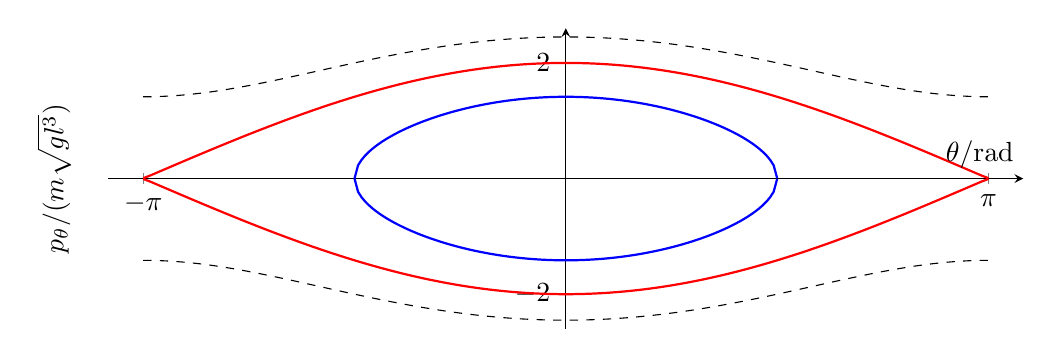
\begin{tikzpicture}
\begin{axis}[width=13.2cm,height=5.4cm,xlabel={$\theta/\unit{rad}$},ylabel={$p_\theta/(m\sqrt{gl^3})$},
 xmin=-3.4,xmax=3.4,ymin=-2.6,ymax=2.6,xtick={-3.14159,0,3.14159},xticklabels={$-\pi$,0,$\pi$},
 samples=121,domain=-pi:pi,axis lines=middle,
 ylabel style={at={(axis description cs:-0.03,0.5)},anchor=south,rotate=90}]
\addplot[blue,thick,domain=-1.570796:1.570796] {sqrt(max(0,2*cos(deg(x))))};
\addplot[blue,thick,domain=-1.570796:1.570796] {-sqrt(max(0,2*cos(deg(x))))};
\addplot[red,thick] {sqrt(2*(1+cos(deg(x))))};
\addplot[red,thick] {-sqrt(2*(1+cos(deg(x))))};
\addplot[black,dashed] {sqrt(2*(2+cos(deg(x))))};
\addplot[black,dashed] {-sqrt(2*(2+cos(deg(x))))};
\end{axis}
    \label{pendulum-phase-portrait}
\end{tikzpicture}

% 排斥 Coulomb 轨道。两条渐近线交于 (0,b)，正焦点 O 为力心。
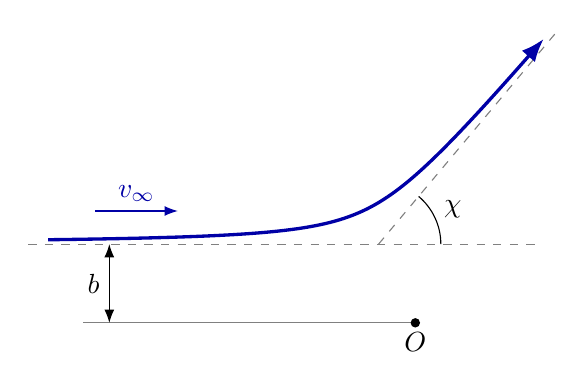
\begin{tikzpicture}[>=Latex]
    \label{rutherford-impact}
    \def\halfAngle{25}
    \coordinate (origin) at ({tan(\halfAngle)},0);
    \coordinate (crossing) at (0,1);
    \draw[gray,dashed] (-4.45,1) -- (2.05,1);
    \draw[gray,dashed] (crossing) -- ++(2.3,{2.3*tan(2*\halfAngle)});
    \draw[gray] (-3.75,0) -- (origin);
    \draw[<->] (-3.42,0) -- node[left] {$b$} (-3.42,1);
    \fill (origin) circle (1.7pt) node[below] {$O$};
    \draw[->,blue!65!black,very thick,domain=-2.04:1.82,samples=75,variable=\t]
        plot ({(cos(2*\halfAngle)*exp(\t)-exp(-\t))/(2*cos(\halfAngle))},
              {1+sin(\halfAngle)*exp(\t)});
    \draw[->,blue!65!black] (-3.6,1.42) -- node[above] {$v_\infty$} (-2.55,1.42);
    \draw (crossing) ++(.79,0) arc[start angle=0,end angle=2*\halfAngle,radius=.79];
    \path (crossing) ++(\halfAngle:1.04) node {$\chi$};
\end{tikzpicture}

\end{document}
